% 	Name		:: 	sthlm Beamer Theme  HEAVILY based on the hsrmbeamer theme (Benjamin Weiss)
%	Author		:: 	Mark Hendry Olson (mark@hendryolson.com)
%	Created		::	2013-07-31
%	Updated		::	June 18, 2015 at 08:45
%	Version		:: 	1.0.2
%	Email		:: 	hendryolson@gmail.com
%	Website		:: 	http://v42.com
%
% 	License		:: 	This file may be distributed and/or modified under the
%                  	GNU Public License.
%
%	Description	::	This presentation is a demonstration of the sthlm beamer
%					theme, which is HEAVILY based on the HSRM beamer theme created by Benjamin Weiss
%					(benjamin.weiss@student.hs-rm.de), which can be found on GitHub
%					<https://github.com/hsrmbeamertheme/hsrmbeamertheme>.


%-=-=-=-=-=-=-=-=-=-=-=-=-=-=-=-=-=-=-=-=-=-=-=-=
%
%        LOADING DOCUMENT
%
%-=-=-=-=-=-=-=-=-=-=-=-=-=-=-=-=-=-=-=-=-=-=-=-=

\documentclass[newPxFont]{beamer}
\usetheme{sthlm}
%\usecolortheme{sthlmv42}

%-=-=-=-=-=-=-=-=-=-=-=-=-=-=-=-=-=-=-=-=-=-=-=-=
%        LOADING PACKAGES
%-=-=-=-=-=-=-=-=-=-=-=-=-=-=-=-=-=-=-=-=-=-=-=-=
\usepackage[utf8]{inputenc}
\usepackage[T1]{fontenc}

\usepackage{chronology}
\usepackage{subfigure}
\usepackage{color} %color in white text in chronologie


%\definecolor{Blue}{rgb}{0,111,174}

\renewcommand{\event}[3][e]{%
  \pgfmathsetlength\xstop{(#2-\theyearstart)*\unit}%
  \ifx #1e%
    \draw[fill=black,draw=none,opacity=0.5]%
      (\xstop, 0) circle (.2\unit)%
      node[opacity=1,rotate=45,right=.2\unit] {#3};%
  \else%
    \pgfmathsetlength\xstart{(#1-\theyearstart)*\unit}%
    \draw[fill=black,draw=none,opacity=0.5,rounded corners=.1\unit]%
      (\xstart,-.1\unit) rectangle%
      node[opacity=1,rotate=45,right=.2\unit] {#3} (\xstop,.1\unit);%
  \fi}%

\DeclareUnicodeCharacter{00A0}{~}
%-=-=-=-=-=-=-=-=-=-=-=-=-=-=-=-=-=-=-=-=-=-=-=-=
%        BEAMER OPTIONS
%-=-=-=-=-=-=-=-=-=-=-=-=-=-=-=-=-=-=-=-=-=-=-=-=

%\setbeameroption{show notes}

%-=-=-=-=-=-=-=-=-=-=-=-=-=-=-=-=-=-=-=-=-=-=-=-=
%
%	PRESENTATION INFORMATION
%
%-=-=-=-=-=-=-=-=-=-=-=-=-=-=-=-=-=-=-=-=-=-=-=-=

\title{L'hybridation de la \\modelisation spatiale \\et de la prospective territoriale}
\subtitle{est-elle soluble dans le Steampunk ?}
%\date{\small{\jobname}}
%\date{\today}
\date{14 Novembre 2018}
\author{\texttt{Etienne DELAY}}
\institute{UR GREEN}

\hypersetup{
pdfauthor = {Etienne DELAY},
pdfsubject = {Séminaire " Prospective territoriale et modelisation "},
pdfkeywords = {modelisation, simulation, prospective},
pdfmoddate= {D:\pdfdate},
pdfcreator = {}
}

\begin{document}

%-=-=-=-=-=-=-=-=-=-=-=-=-=-=-=-=-=-=-=-=-=-=-=-=
%
%	TITLE PAGE
%
%-=-=-=-=-=-=-=-=-=-=-=-=-=-=-=-=-=-=-=-=-=-=-=-=

\maketitle

%\begin{frame}[plain]
%	\titlepage
%\end{frame}

%-=-=-=-=-=-=-=-=-=-=-=-=-=-=-=-=-=-=-=-=-=-=-=-=
%
%	TABLE OF CONTENTS: OVERVIEW
%
%-=-=-=-=-=-=-=-=-=-=-=-=-=-=-=-=-=-=-=-=-=-=-=-=
%\section*{Overview}
%\begin{frame}{Overview}
%% For longer presentations use hideallsubsections option
%\tableofcontents[hideallsubsections]
%\end{frame}

\section{Le Steampunk ?}

%-=-=-=-=-=-=-=-=-=-=-=-=-=-=-=-=-=-=-=-=-=-=-=-=
%	FRAME: LE STEAMPUNK, LE MYSTERE D'UN TITRE
%-=-=-=-=-=-=-=-=-=-=-=-=-=-=-=-=-=-=-=-=-=-=-=-=

\begin{frame}[c]{Lever les ambiguités : Steampunk ? }
\vspace{-1cm}
Proto-science-fictions, mettant en scène des pionniers scientifiques uchronique dans des decores victorien.
\begin{figure}
  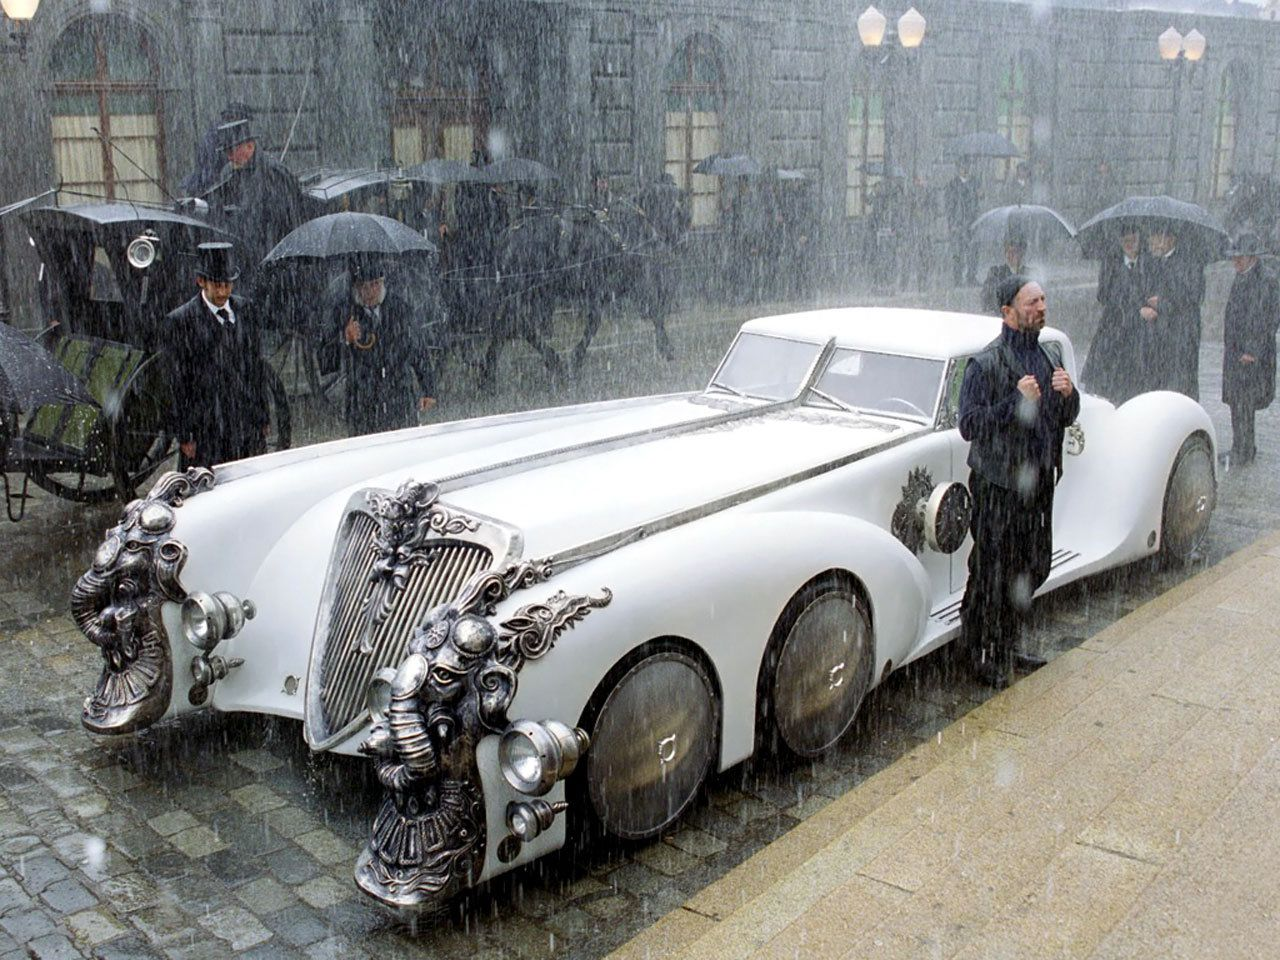
\includegraphics[height=6cm]{img/a_steampunk_car.jpg}
\end{figure}
\end{frame}

\begin{frame}[c]{Modelisation, prospective et Steampunk?}
\vspace{-1cm}
Reviens à questionner le status de l'un par rapport à l'autre
\begin{figure}
  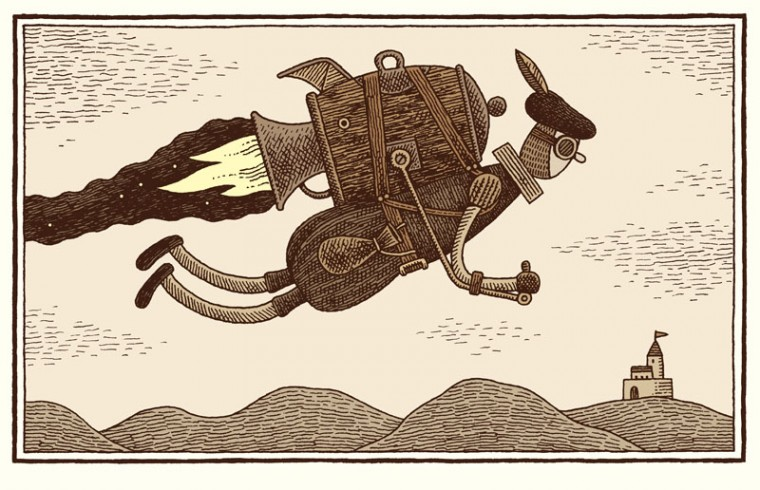
\includegraphics[height=6cm]{img/a_Tom-Gauld-jetpack.jpg}
\end{figure}
\end{frame}

\section{Epistemologie de la\\ modelisation : le domaine}

%-=-=-=-=-=-=-=-=-=-=-=-=-=-=-=-=-=-=-=-=-=-=-=-=
%	FRAME: EPISTEMOLOGIE DE LA MODELISATION
%-=-=-=-=-=-=-=-=-=-=-=-=-=-=-=-=-=-=-=-=-=-=-=-=

\begin{frame}[c]{Du Système au modèle, tentatives de thérorisation}
\vspace{-1em}
\begin{quote}
  \enquote{<<le terme de \textbf{modèle} a la même signification que celui de concept ou d'hypothèse ou d'analogie [...], un modèle est une abstraction qui simplifie le système réel étudié [...] pour se focaliser sur les aspects qui intéressent le modélisateur et qui définissent les problématiques du modèle.>>}
\end{quote}
\hspace*{\fill}\textsc{Coquillard et Hill 1997, p.7}
\vspace{-0.5em}
\begin{figure}
 	\centering
 		\subfigure{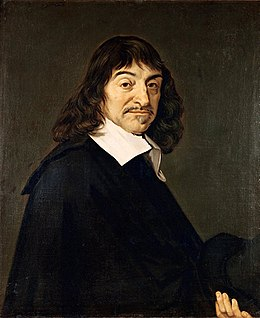
\includegraphics[height=3cm]{img/a_descartes.jpg}}\hspace{0.2em}%%descartes
    \subfigure{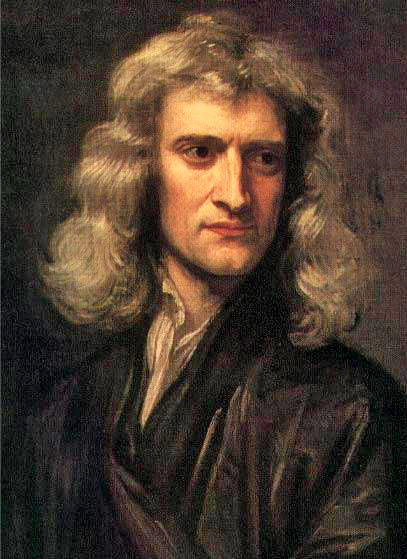
\includegraphics[height=3cm]{img/a_newton.jpg}}\hspace{0.2em}%% newton
 		\subfigure{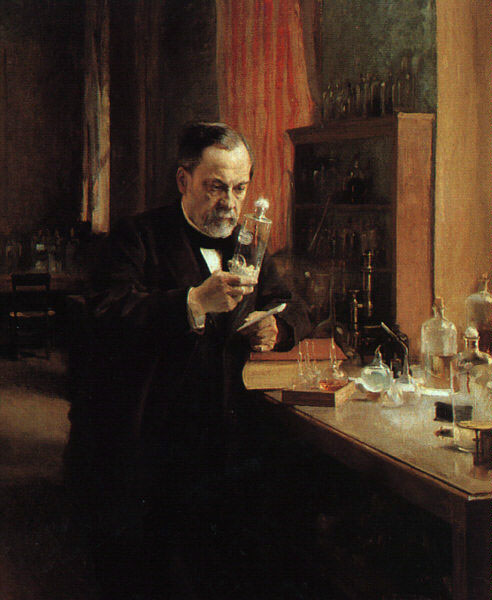
\includegraphics[height=3cm]{img/a_pasteur.jpg}}\hspace{0.2em}%%pasteur
    \subfigure{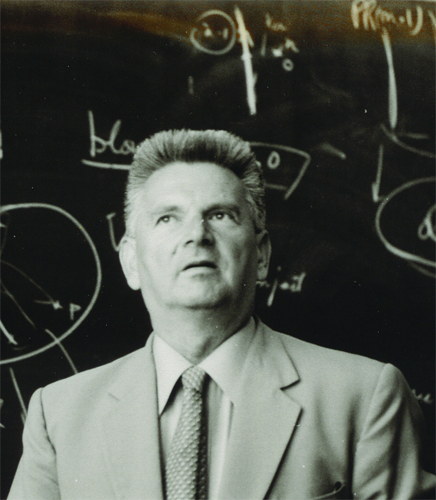
\includegraphics[height=3cm]{img/a_thom.png}}%%thom
\end{figure}
\end{frame}

\begin{frame}[c]{Du Système au modèle, tentatives de thérorisation}
\vspace{-1em}
\begin{quote}
  \enquote{<<la \textbf{théorisation} [...] est liée à la possibilité de plonger le réel dans un virtuel imaginaire, doté de propriétés génératives, qui permettent de faire des prévisions.>>}
\end{quote}
\hspace*{\fill}\textsc{Thom 2009, p. 91}
\vspace{-0.5em}
\begin{figure}
 	\centering
 		\subfigure{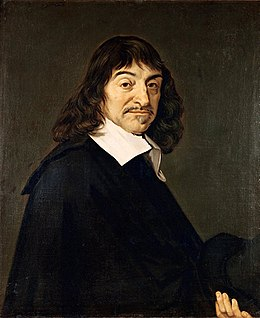
\includegraphics[height=3cm]{img/a_descartes.jpg}}\hspace{0.2em}%%descartes
    \subfigure{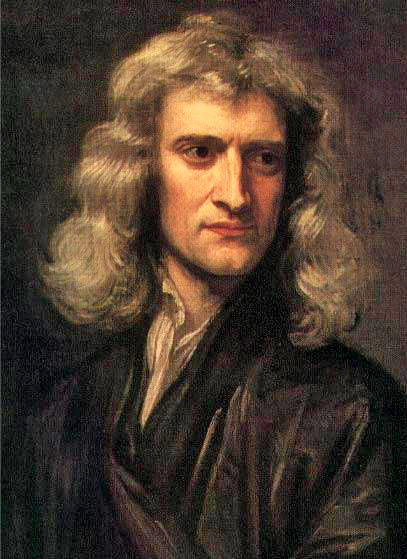
\includegraphics[height=3cm]{img/a_newton.jpg}}\hspace{0.2em}%% newton
 		\subfigure{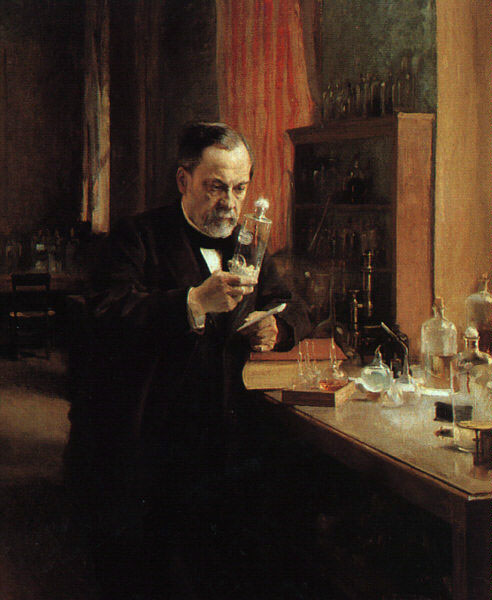
\includegraphics[height=3cm]{img/a_pasteur.jpg}}\hspace{0.2em}%%pasteur
    \subfigure{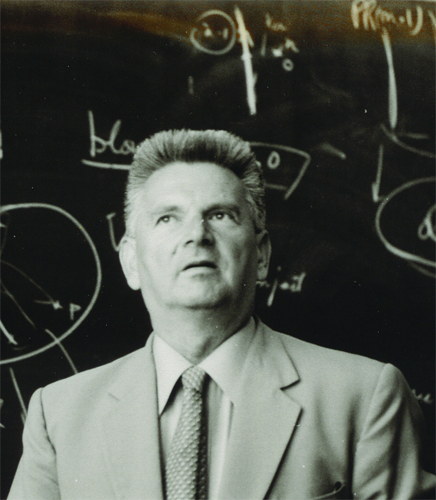
\includegraphics[height=3cm]{img/a_thom.png}}%%thom
\end{figure}
\end{frame}

\begin{frame}[c]{Des modèles pour la recherche de formes}
\vspace{-1em}
\begin{quote}
  \enquote{Peut-on, dans un paysage de phénomènes, reconnaître un objet ou une chose si l'on n'en a pas au préalable le concept ? C'est aussi simple que ça. Si l'on n'a pas le concept d'un objet, on ne le reconnaîtra pas. [...] La possibilité de reconnaître un être en général, une entité dans un paysage empirique, est toujours à mon avis subordonnée à une conceptualisation}
\end{quote}
\hspace*{\fill}\textsc{Thom 2009, p.93}
\vspace{-0.5em}
\begin{figure}
 
\includegraphics[height=3cm]{img/a_rorschach.png}
\end{figure}
\end{frame}

\section{Epistemologie de la\\ modelisation : controverse}
%-=-=-=-=-=-=-=-=-=-=-=-=-=-=-=-=-=-=-=-=-=-=-=-=
%	FRAME: CONTROVERSE
%-=-=-=-=-=-=-=-=-=-=-=-=-=-=-=-=-=-=-=-=-=-=-=-=
\begin{frame}[c]{Le réductionnisme}
\vspace{-1em}
\begin{quote}
  \enquote{<<Consiste à fragmenter des systèmes complexes en éléments plus simples à étudier.>>}
\end{quote}
\hspace*{\fill}\textsc{Wiktionnaire 2018}
\vspace{-0.5em}
\begin{figure}
 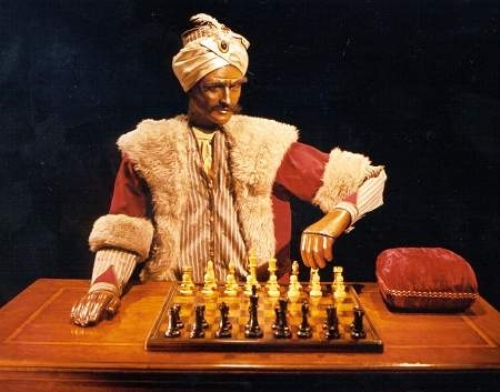
\includegraphics[height=3cm]{img/a_turc_automaton.jpg}
\end{figure}
\end{frame}

\begin{frame}[c]{Le holisme}
\vspace{-1em}
\begin{quote}
  \enquote{<<consiste à considérer les phénomènes individuels ou particuliers comme faisant partie de la totalité dans laquelle ils s’inscrivent.>>}
\end{quote}
\hspace*{\fill}\textsc{Wiktionnaire 2018}
\vspace{-0.5em}
\begin{figure}
 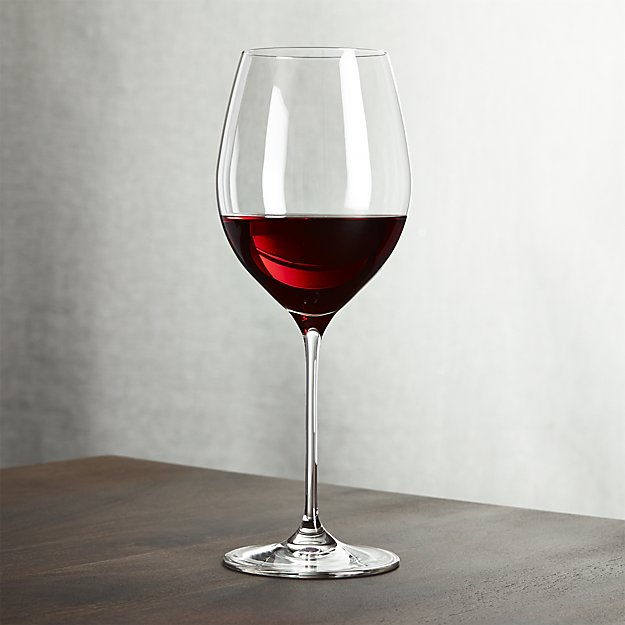
\includegraphics[height=3cm]{img/a_wine.jpeg}
\end{figure}
\end{frame}

\begin{frame}[c]{Une $3^{\`eme}$ voie : la \textit{complexité}}
\vspace{-1em}
\begin{quote}
  \enquote{TODO}
\end{quote}
\hspace*{\fill}\textsc{Thom 2009, p.93}
\vspace{-0.5em}
\begin{figure}
 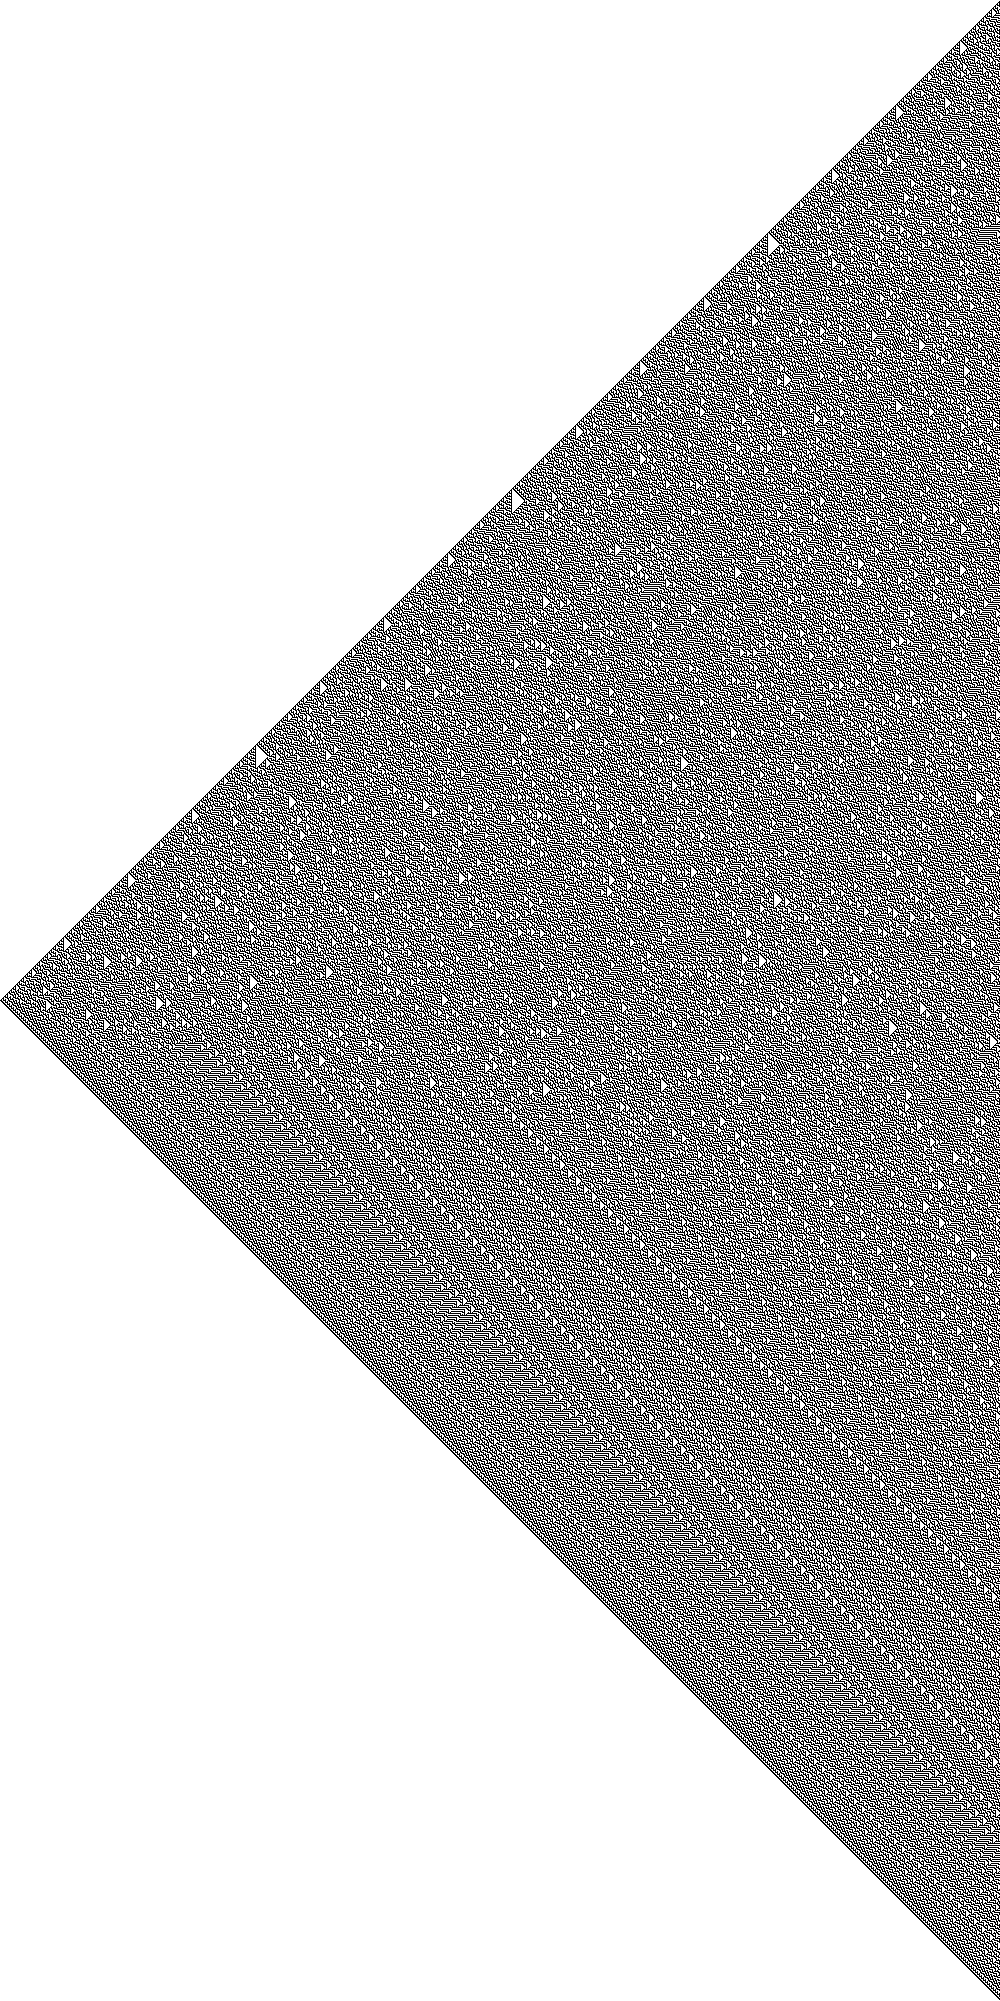
\includegraphics[angle=90,height=5cm]{img/a_rule_wolfram.png}
\end{figure}
\end{frame}

\begin{frame}[c]{Gardes fous}
\vspace{-1em}
\begin{quote}
  \enquote{<<Cela n'implique pas que l'on prenne définitivement parti pour le holisme (\textsc{Valade 2001}), contre l'individualisme méthodologique (\textsc{Boudon 2004}), mais cela implique qu'on garde l'un et l'autre en mémoire comme gardes fous de l'autre>>}
\end{quote}
\hspace*{\fill}\textsc{Pumain 2003 p.26}
\vspace{-0.5em}
\begin{figure}
 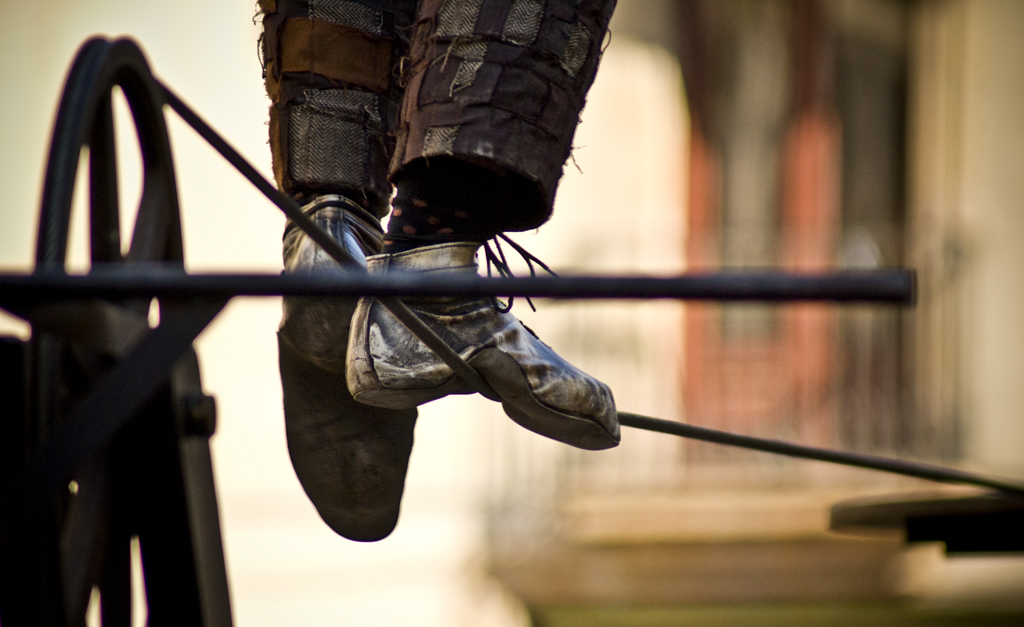
\includegraphics[height=3cm]{img/a_Funambule.jpg}
\end{figure}
\end{frame}

\section{Epistemologie de la\\ modelisation : simulation}
%-=-=-=-=-=-=-=-=-=-=-=-=-=-=-=-=-=-=-=-=-=-=-=-=
%	FRAME: CONTROVERSE
%-=-=-=-=-=-=-=-=-=-=-=-=-=-=-=-=-=-=-=-=-=-=-=-=

\begin{frame}[c]{A base de popopop !}
\vspace{-2em}
\begin{figure}
 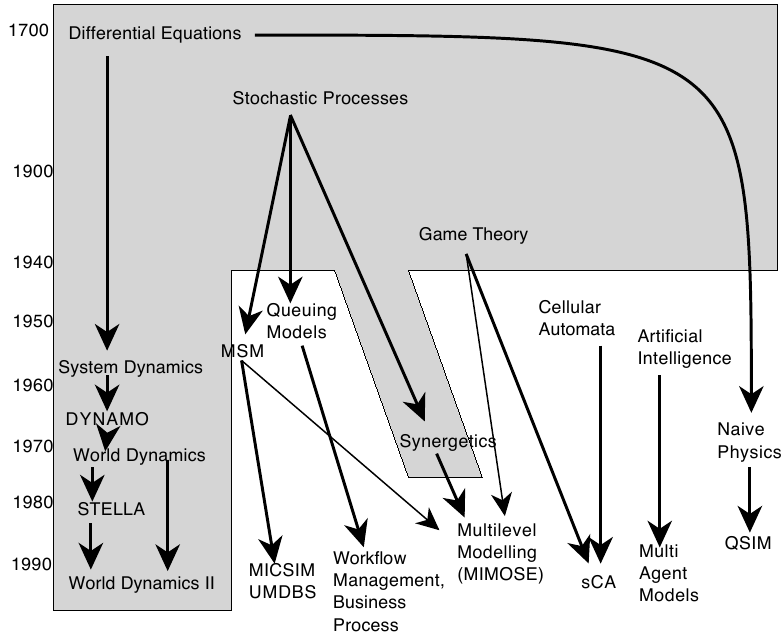
\includegraphics[height=6cm]{img/a_troitzsch_1997.png}
\end{figure}
\vspace{-0.8em}
\small{Le développement de l'approche de simulation contemporaine en sciences sociales (d'après \textsc{Troitzsch} 1997). La partie grise représente les modèles à base d'équation, la partie blanche les modèles à base d'objets, d'événements, ou d'agents}.

\end{frame}


\begin{frame}[c]{Un parcours interdisciplinaire}

\vspace{-1cm}
\begin{center}\begin{chronology}[2]{2004}{2018}{0.95\textwidth}
\event[\decimaldate{1}{9}{2004}]{\decimaldate{1}{6}{2006}}{\color{lightgray}L1 \& L2 de Biologie}
\event[\decimaldate{1}{9}{2006}]{\decimaldate{1}{6}{2008}}{\color{lightgray}BTSA -- GPN }
\event[\decimaldate{1}{9}{2008}]{\decimaldate{1}{6}{2011}}{L3 - M1- M2 -- Géographie}
\event[\decimaldate{1}{9}{2009}]{\decimaldate{1}{6}{2011}}{DEUST "Intranet et SGBD"}
\event[\decimaldate{1}{9}{2011}]{\decimaldate{1}{6}{2015}}{\color{lightgray}Doctorat de Géographie}
\event{\decimaldate{10}{6}{2015}}{\cRed{\small{\color{lightgray}Soutenance de doctorat}}}
\event[\decimaldate{1}{9}{2015}]{\decimaldate{1}{2}{2018}}{\color{lightgray}Postdoctorats}
\end{chronology}
\end{center}

\vspace{1em}

\begin{figure}
 	\centering
 		\subfigure{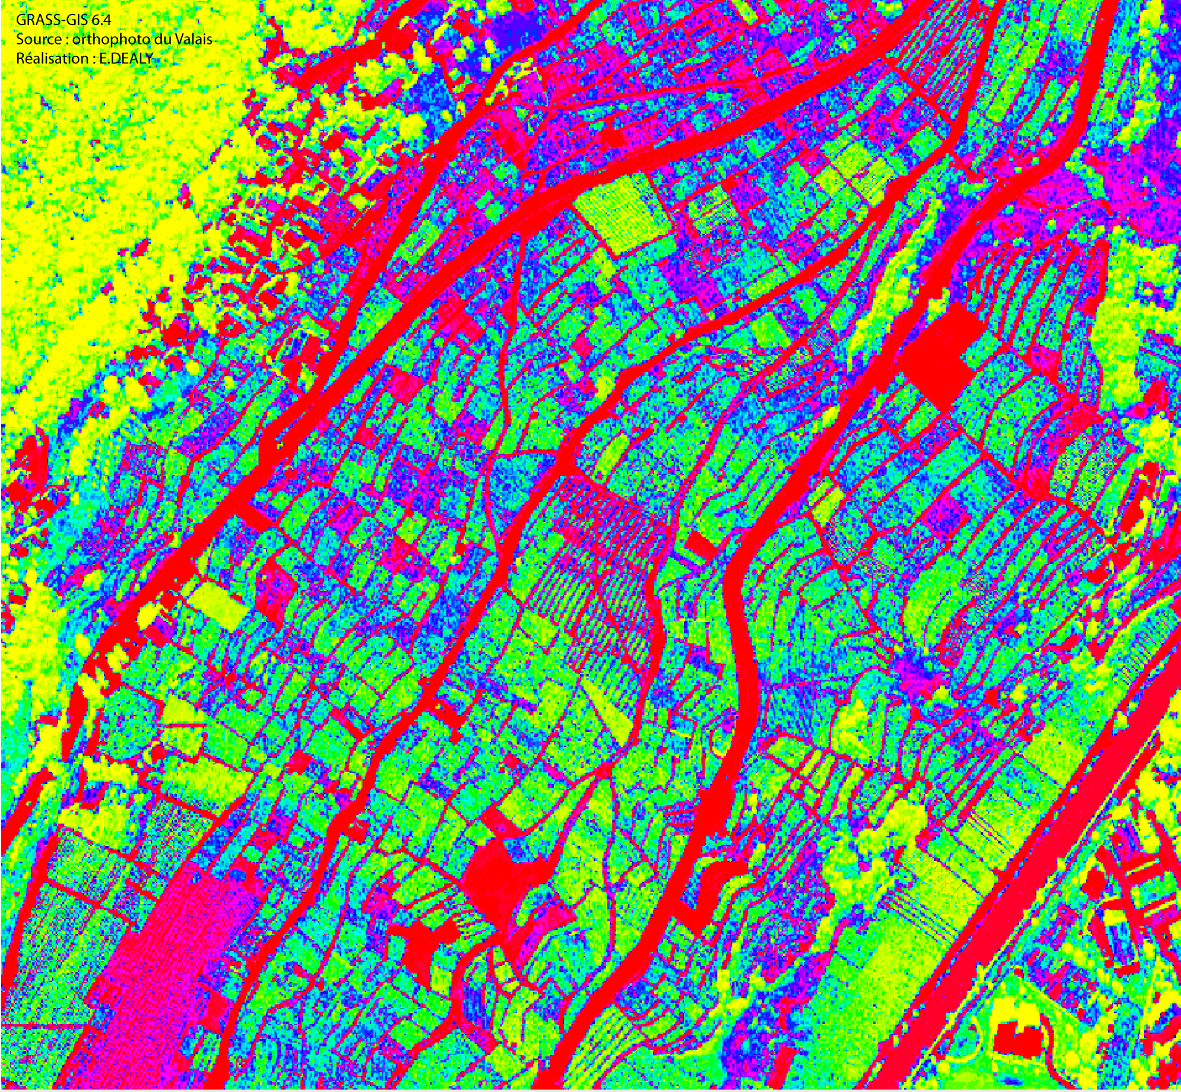
\includegraphics[height=3cm]{img/teledec}}\hspace{1em}%image teledec
 		\subfigure{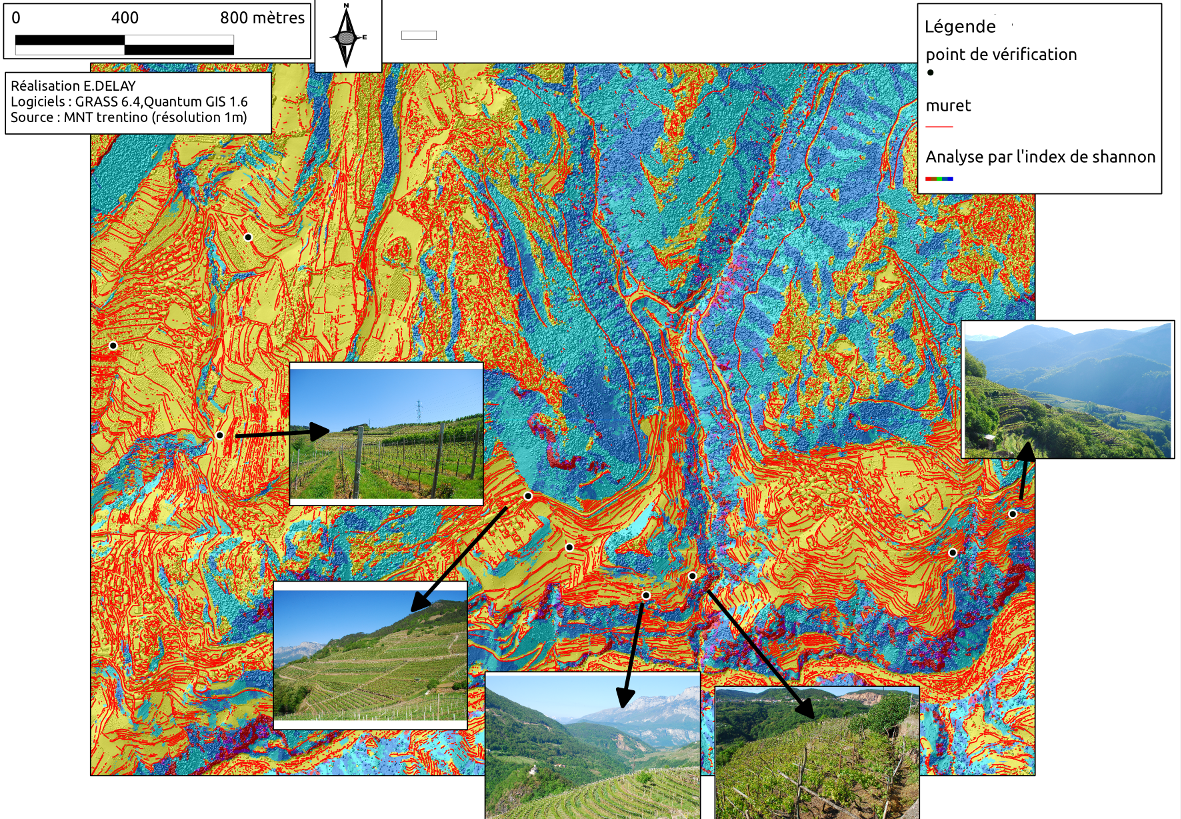
\includegraphics[height=3cm]{img/lidar}}%image Lidar
\end{figure}

\end{frame}


\begin{frame}[c]{Un parcours interdisciplinaire}

\vspace{-1cm}
\begin{center}\begin{chronology}[2]{2004}{2018}{0.95\textwidth}
\event[\decimaldate{1}{9}{2004}]{\decimaldate{1}{6}{2006}}{\color{lightgray}L1 \& L2 de Biologie}
\event[\decimaldate{1}{9}{2006}]{\decimaldate{1}{6}{2008}}{\color{lightgray}BTSA -- GPN }
\event[\decimaldate{1}{9}{2008}]{\decimaldate{1}{6}{2011}}{\color{lightgray}L3 - M1- M2 -- Géographie}
\event[\decimaldate{1}{9}{2009}]{\decimaldate{1}{6}{2011}}{\color{lightgray}DEUST "Intranet et SGBD"}
\event[\decimaldate{1}{9}{2011}]{\decimaldate{1}{6}{2015}}{Doctorat de Géographie}
\event{\decimaldate{10}{6}{2015}}{\cRed{\small{Soutenance de doctorat}}}
\event[\decimaldate{1}{9}{2015}]{\decimaldate{1}{2}{2018}}{Postdoctorats}
\end{chronology}
\end{center}
\vspace{-1em}
\begin{small}
  \begin{itemize}
    \item \textbf{Thèse de Doctorat} : Sous la direction de É. \textsc{Rouvellac}, N. \textsc{Becu} et P. \textsc{Allée} $\rightarrow$ comportements individuels (SMA) et dynamiques spatiales agricoles (4 articles + une thèse). 
\includegraphics[width=0.5cm]{img/d_italie}~
\includegraphics[width=0.5cm]{img/d_france}
    \item \textbf{Postdoc 1} : Sous la direction de J. \textsc{Linton} $\rightarrow$ le partage de l'eau, un système complexe (2 articles + 1 chapitre d'ouvrage) 
\includegraphics[width=0.5cm]{img/d_france}
    \item \textbf{Postdoc 2} : Sous la direction de J.-L. \textsc{Peiry} $\rightarrow$ co-construction de données sur la résilience des SES Sahelien ~
\includegraphics[width=0.5cm]{img/d_senegal}
  \end{itemize}
\end{small}

\end{frame}


%-=-=-=-=-=-=-=-=-=-=-=-=-=-=-=-=-=-=-=-=-=-=-=-=
%
%	SECTION: ACTIVITE DE RECHERCHE
%
%-=-=-=-=-=-=-=-=-=-=-=-=-=-=-=-=-=-=-=-=-=-=-=-=

\subsection{Activites de recherche}
%-=-=-=-=-=-=-=-=-=-=-=-=-=-=-=-=-=-=-=-=-=-=-=-=
%	FRAME: AXE 1 Dynamiques des Socio-ecosystèmes comme porte d'entrer
%-=-=-=-=-=-=-=-=-=-=-=-=-=-=-=-=-=-=-=-=-=-=-=-=

\begin{frame}{Axe 1 : Facilitation, coopération et production d'espace}
	\vspace{-2em}
	\small{
		\begin{block}{\textsc{Questionnements thematiques}}
			Y a-t-il des conditions favorisant la coopération ? Peut-on faciliter l'émergence de la gestion collective des ressources naturelles ?
		\end{block}
	}
  \vspace{-1em}
	\begin{itemize}
    \item Les interactions sociales → traces dans les territoires (4 articles),
		\item L'hétérogénité spatiale / temporelle des ressources → interactions sociales (1 article)
	\end{itemize}
  \vspace{-1em}
  \begin{figure}
   			\centering
   				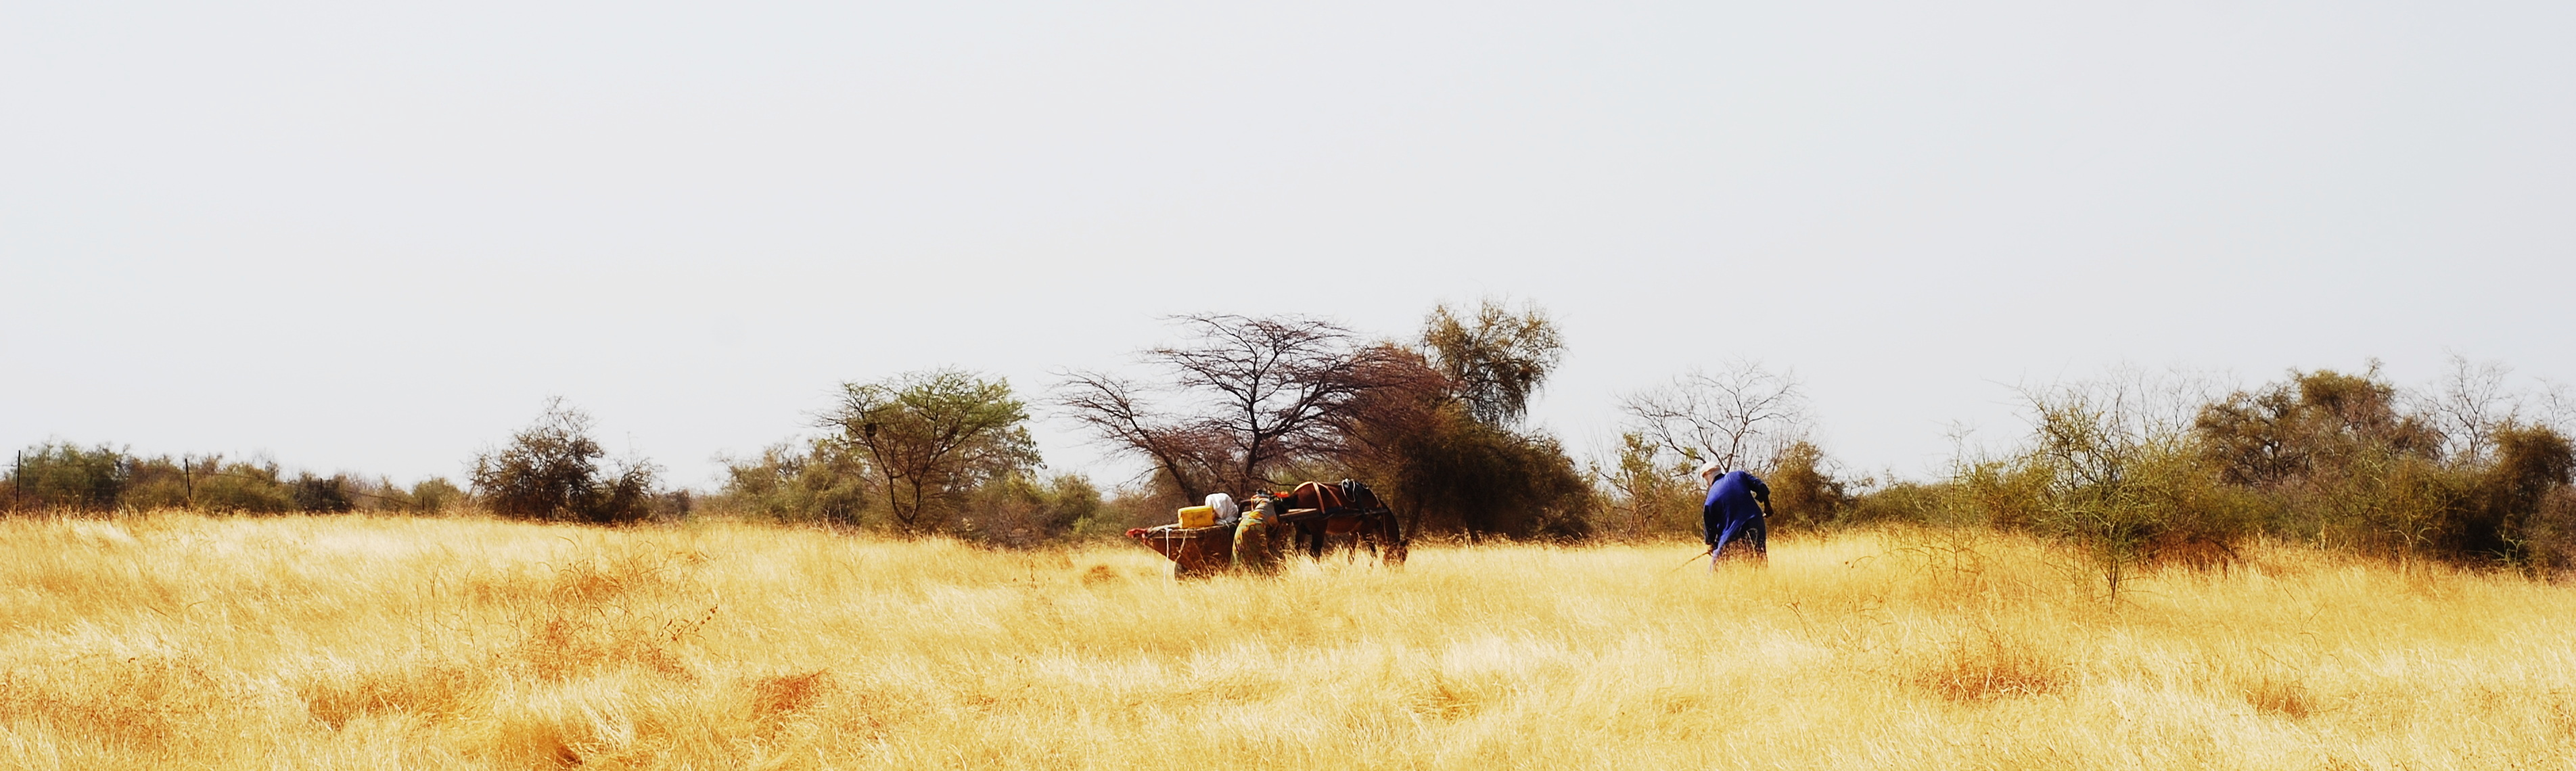
\includegraphics[width=0.95\textwidth]{img/parcelle_gmv}
  \end{figure}
\end{frame}


%-=-=-=-=-=-=-=-=-=-=-=-=-=-=-=-=-=-=-=-=-=-=-=-=
%	FRAME: AXE 2 INTERACTION ET ADAPTATION
%-=-=-=-=-=-=-=-=-=-=-=-=-=-=-=-=-=-=-=-=-=-=-=-=

\begin{frame}{Axe 2 : Modélisation et SMA pour l'accompagnement}
	\vspace{-2em}
	\small{
		\begin{alertblock}{\textsc{Questionnements methodologiques}}
				Modélisation et simulation : outils de \alert{formalisation}, \alert{compréhension} et d'\alert{exploration} des interactions société $\leftrightarrow$ environnement.
		\end{alertblock}
	}
  \vspace{-1em}
	\begin{itemize}
		\item Co-construction et modélisation d'accompagnement
		\begin{itemize}
			\item Doctorat : 6 SMA issus des questionnements des acteurs
			\item LittoSim : défi CNRS → Sim. Participative (Oléron)
      \item Construction d'un jeu de plateau (Nep-tunes)
		\end{itemize}
		\item Approche critique du modèle (positionnement du modèle vis-à-vis des acteurs, des modélisateurs, etc.)
	\end{itemize}
  \vspace{-1em}
	\begin{figure}
 			\centering
 				\subfigure{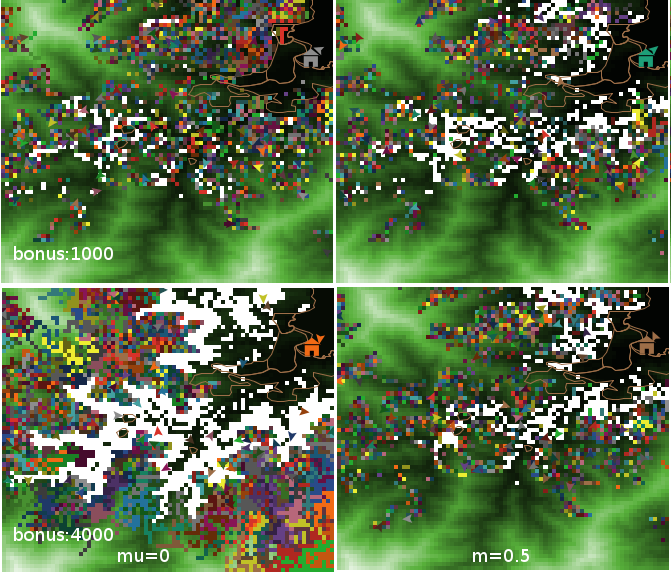
\includegraphics[width=0.3\textwidth]{img/acidityGIS}}
 				\subfigure{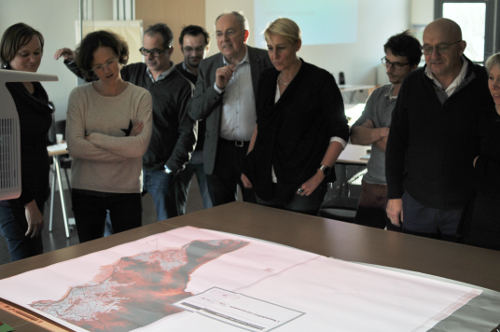
\includegraphics[width=0.3\textwidth]{img/LittoSim}}
        \subfigure{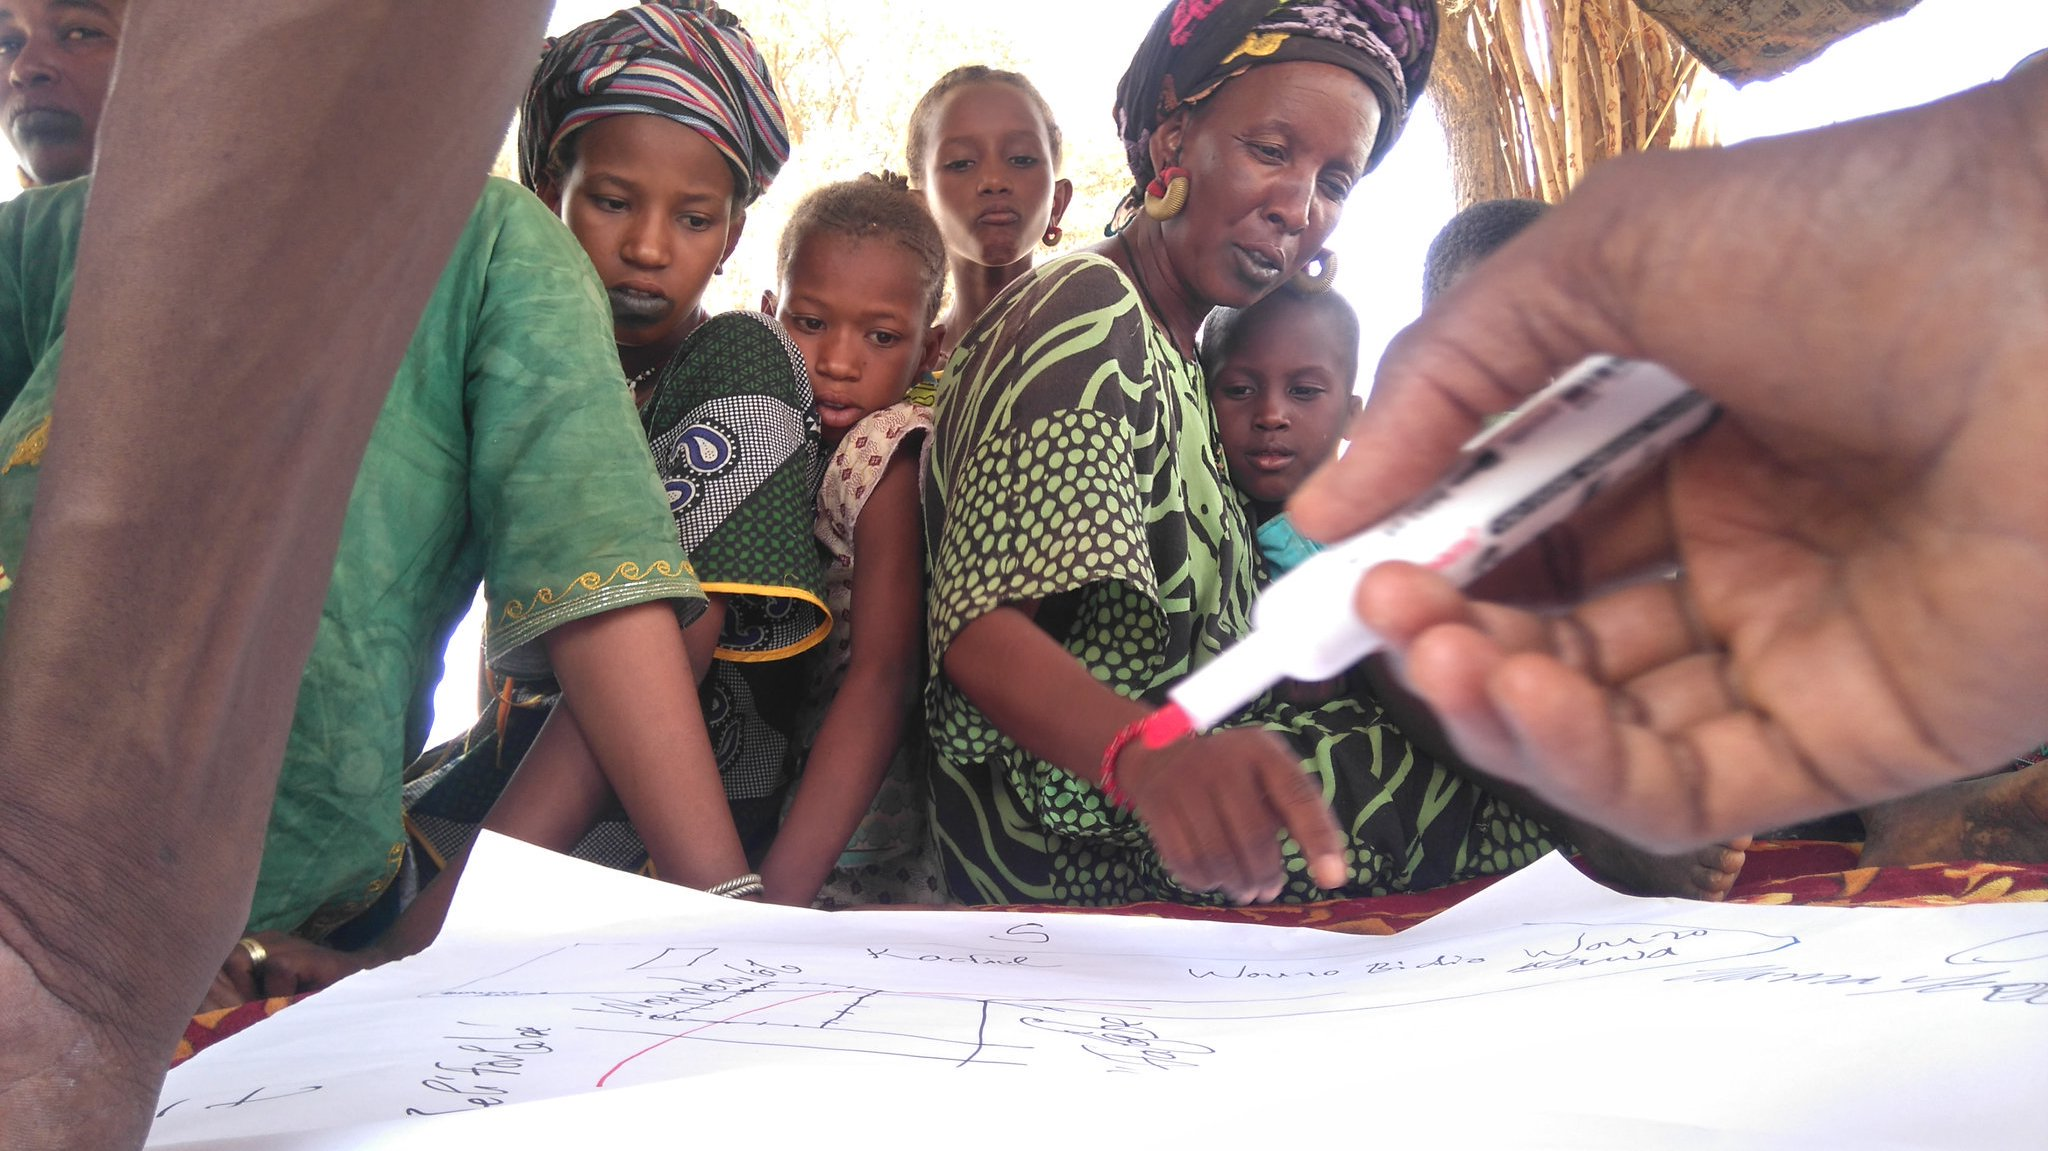
\includegraphics[width=0.3\textwidth]{img/mission_fs}}
	\end{figure}

\end{frame}

%-=-=-=-=-=-=-=-=-=-=-=-=-=-=-=-=-=-=-=-=-=-=-=-=
%	FRAME: APERçU
%-=-=-=-=-=-=-=-=-=-=-=-=-=-=-=-=-=-=-=-=-=-=-=-=

\begin{frame}{Pratique et valorisation de la recherche}
\vspace{-2em}
\begin{itemize}
  \item Implication dans de nombreux projets de recherche : \alert{\color{sthlmBlue}ANR TerViClim}, LACCAVE, ChOICE\textsuperscript{*}, \alert{\color{sthlmBlue}COMMONS}\textsuperscript{*}, LittoSim, \alert{\color{sthlmBlue}ANR \textit{Future Sahel}}.
	\item Des partenariats de recherche à l'international : France, Italie, Allemagne, Maroc, Sénégal, Suède.
	\item Impliqué dans les communautés MAPS\textsuperscript{*}, MISSABMS et 
\includegraphics[width=0.8cm]{img/Logo_OSGeo}.
	\item Travaux interdisciplinaires : économistes, sci. de l'environnement, écologues, géographes et géo-sci., \textit{etc}.
\end{itemize}
\vspace{-2em}
\begin{figure}
 	\centering
 		\subfigure{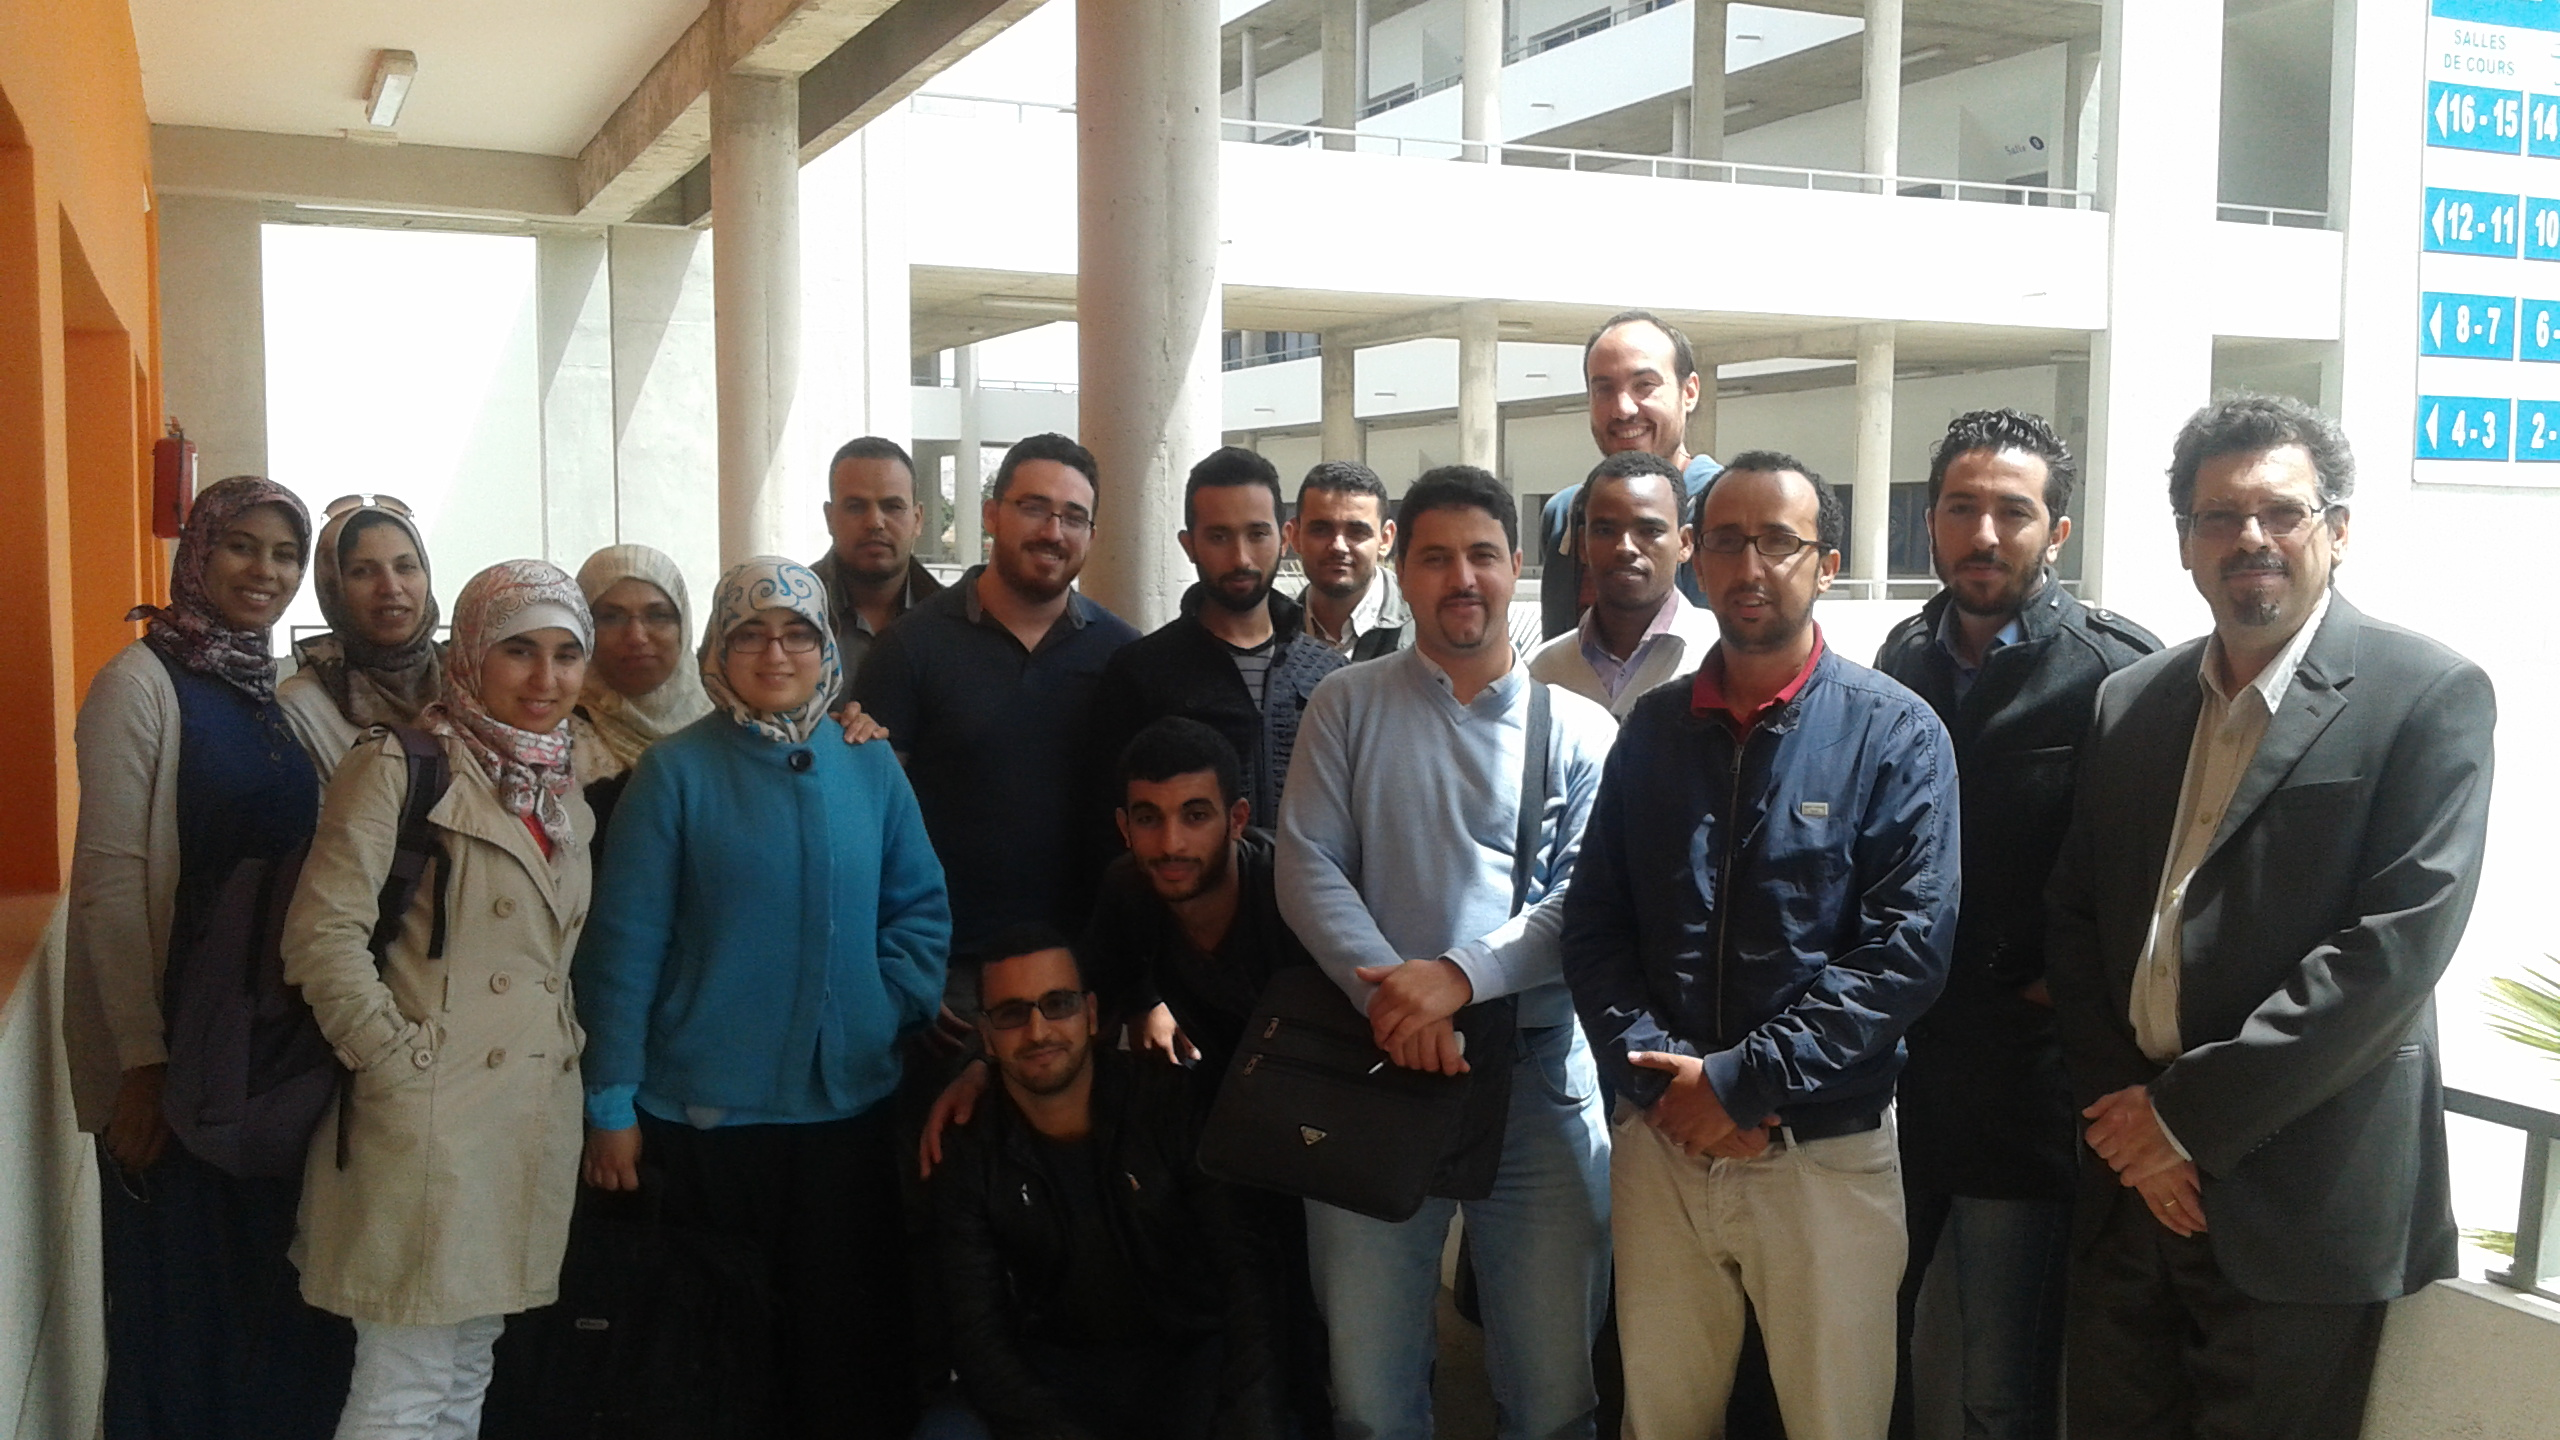
\includegraphics[height=2.25cm]{img/group_agadir}}
 		\subfigure{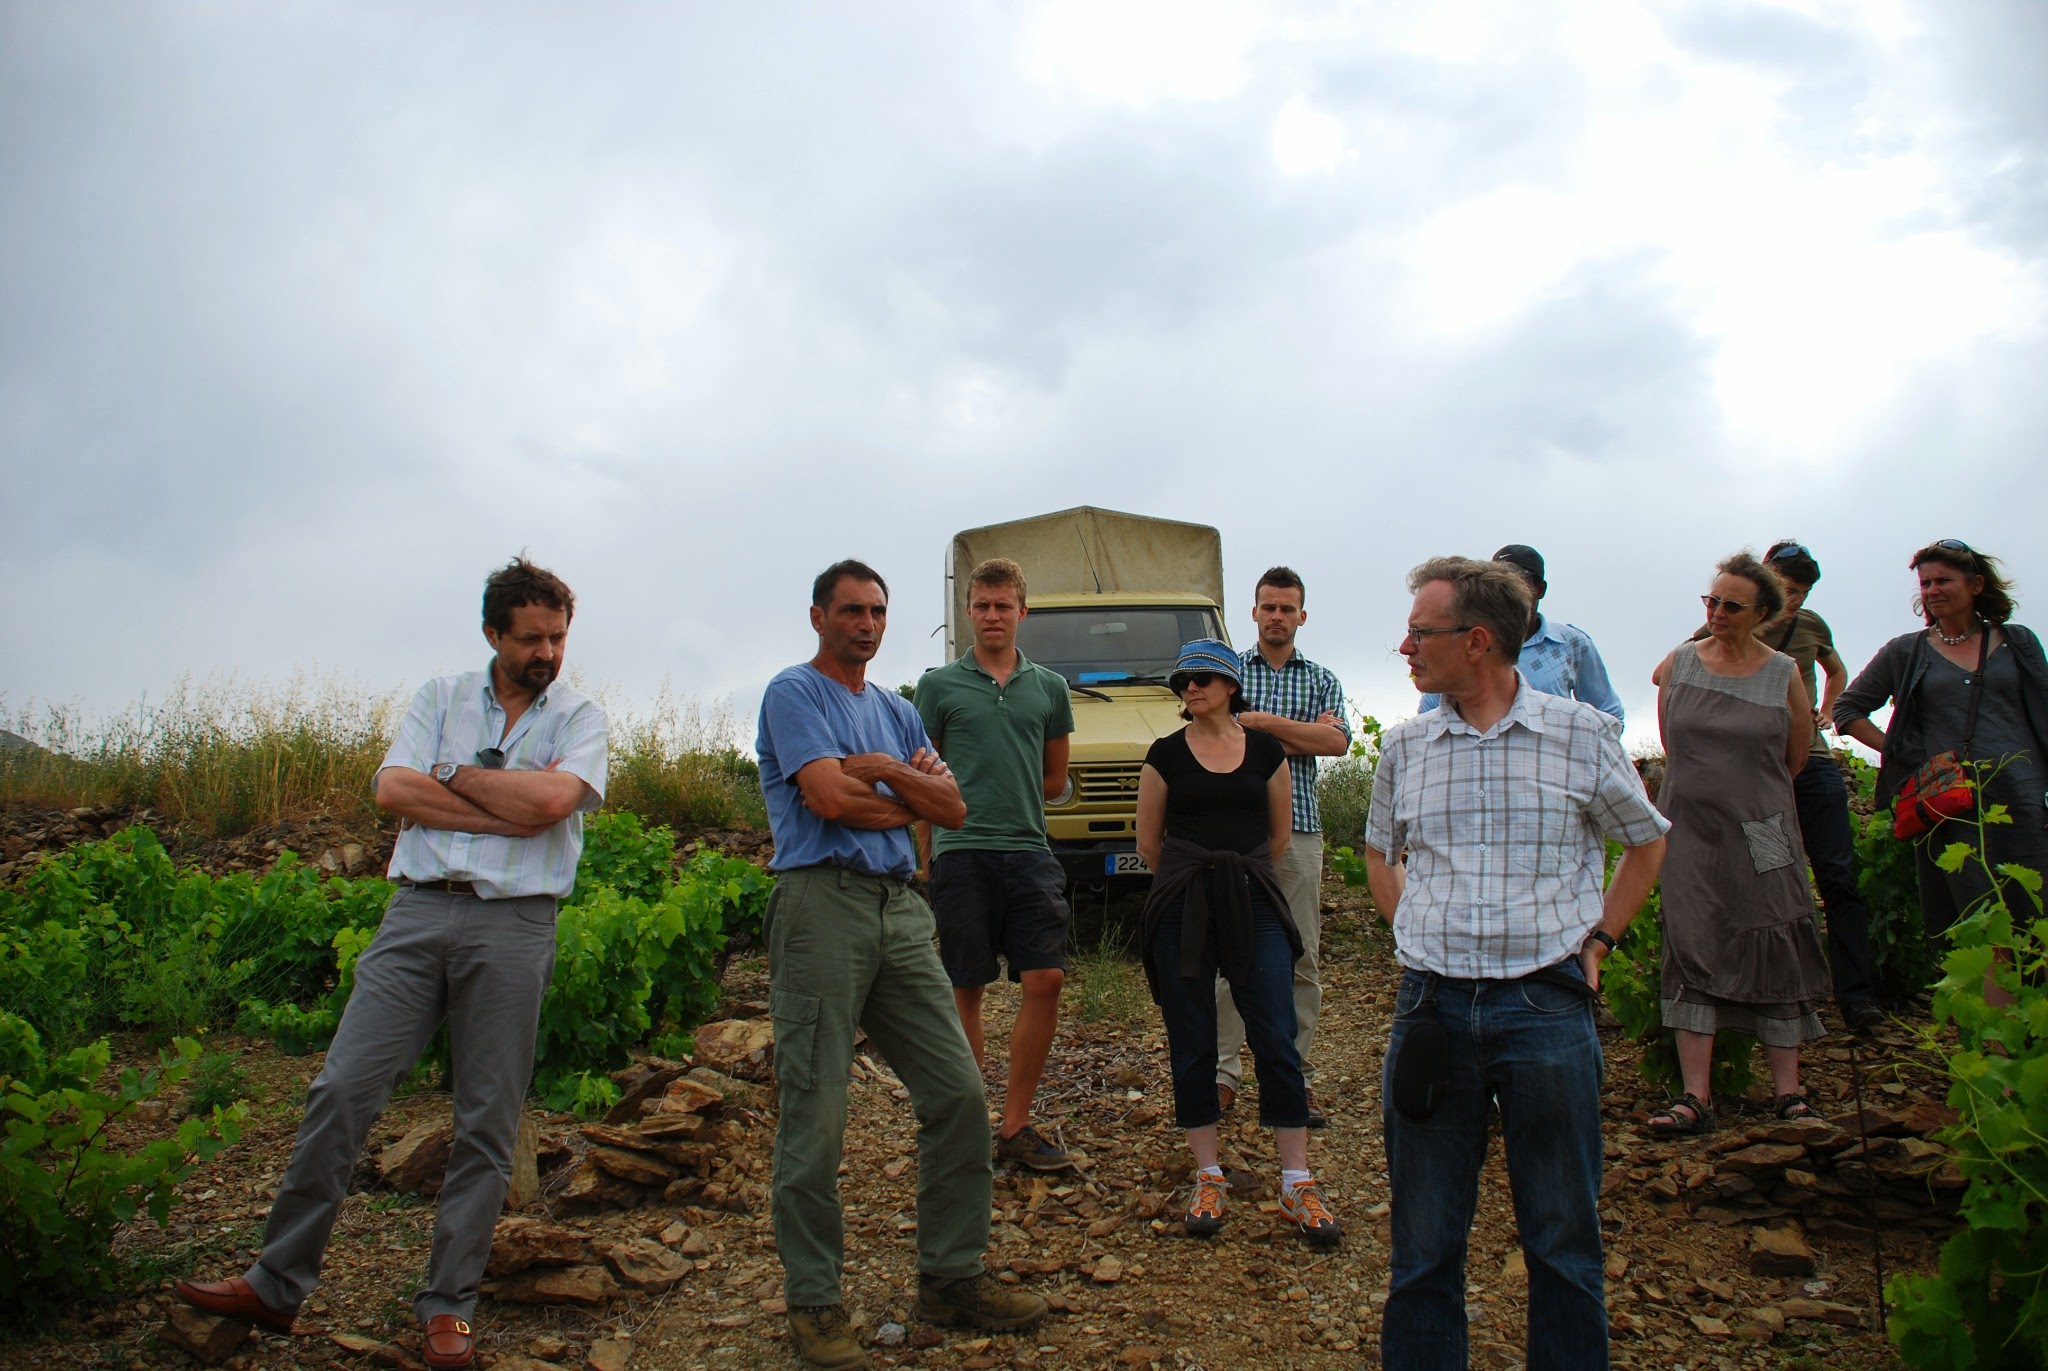
\includegraphics[height=2.25cm]{img/lacave_terrain}}
 		\subfigure{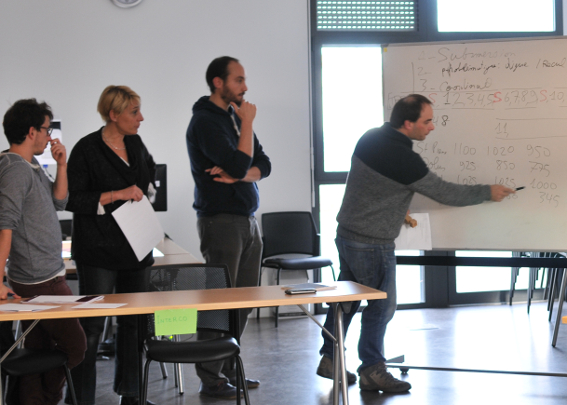
\includegraphics[height=2.25cm]{img/ateliers}}
\end{figure}
\end{frame}

%-=-=-=-=-=-=-=-=-=-=-=-=-=-=-=-=-=-=-=-=-=-=-=-=
%
%	SECTION: VISION DU POSTE ET PROSPECTIVE
%
%-=-=-=-=-=-=-=-=-=-=-=-=-=-=-=-=-=-=-=-=-=-=-=-=

\section{Projet de Recherche \& vision du poste}

%-=-=-=-=-=-=-=-=-=-=-=-=-=-=-=-=-=-=-=-=-=-=-=-=
%	FRAME: LES ATTENTES DU POSTE
%-=-=-=-=-=-=-=-=-=-=-=-=-=-=-=-=-=-=-=-=-=-=-=-=

\begin{frame}{Ma vision du poste}
	\vspace{-2em}

  \begin{figure}
    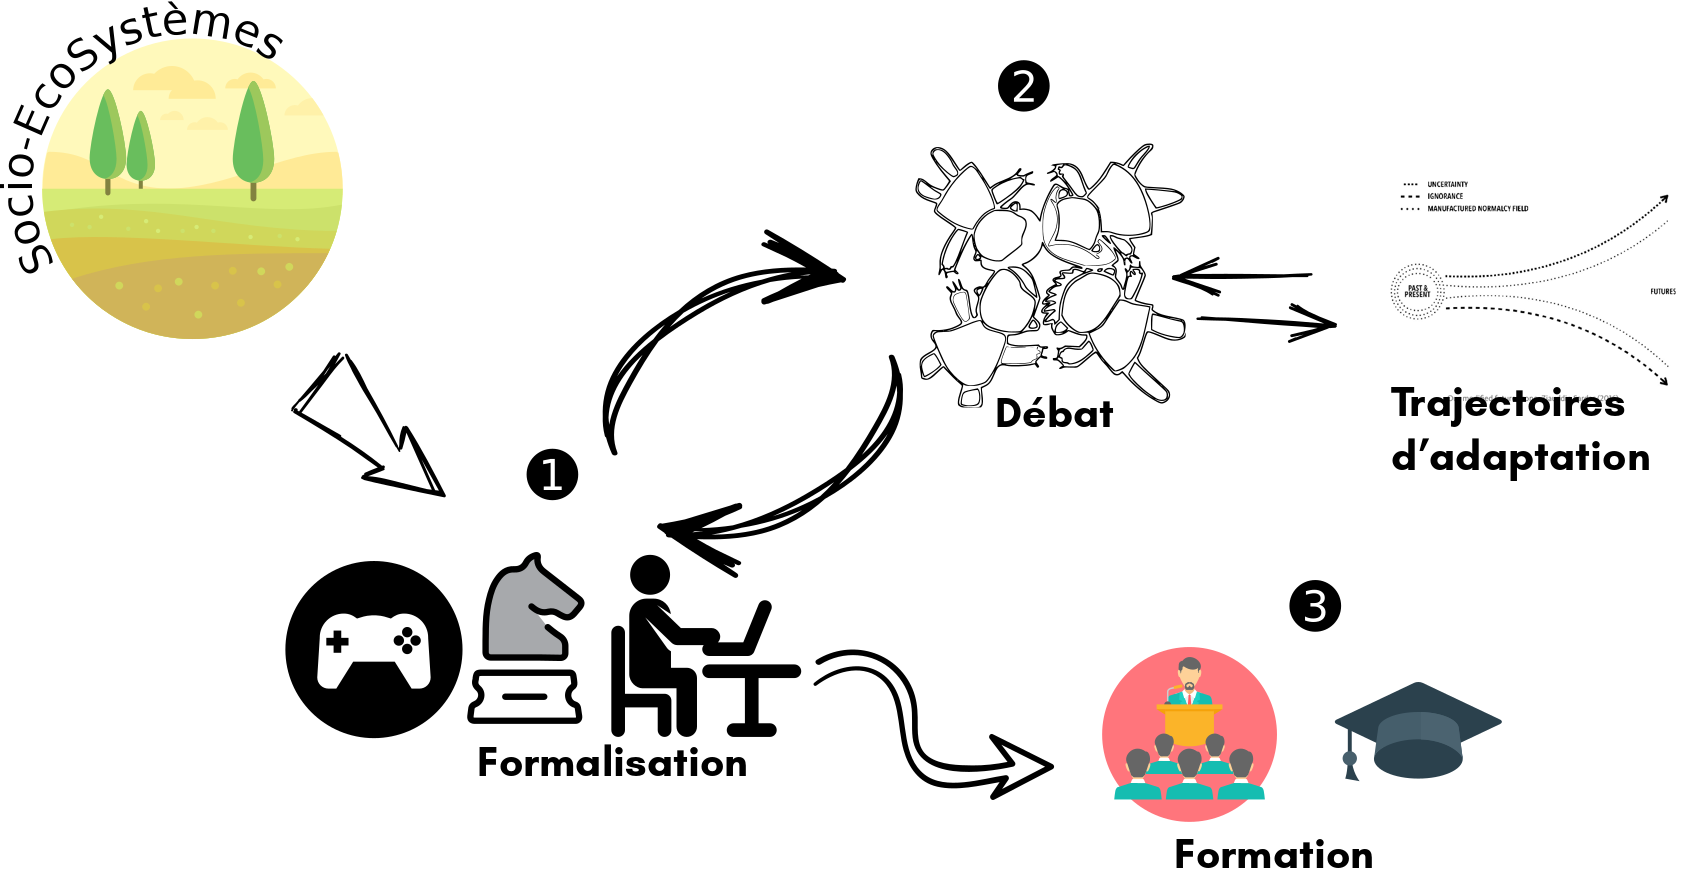
\includegraphics[width=\textwidth]{img/profil_poste}
  \end{figure}
\end{frame}

%-=-=-=-=-=-=-=-=-=-=-=-=-=-=-=-=-=-=-=-=-=-=-=-=
%	FRAME: Mes questionnements
%-=-=-=-=-=-=-=-=-=-=-=-=-=-=-=-=-=-=-=-=-=-=-=-=

\begin{frame}{Questionnement et intégration à l'UR GREEN}
	\vspace{-2em}
  Je suis un \alert{\color{sthlmBlue}géographe} interdiciplinaire, rompu à la modélisation d'accompagnement $\rightarrow$ L'\alert{\color{sthlmBlue}espace} joue un rôle fondamental !
  \begin{block}{\textsc{Mes Questionnements}}
    \begin{enumerate}
      \item Comment les ressources territorialisées influencent-elles les interactions sociales et la constitution de groupes ?
      \item Est-ce que les types de ressources gérées influencent les dynamiques de groupe ?
    \end{enumerate}
	\end{block}
  \vspace{-1em}
  \begin{figure}
    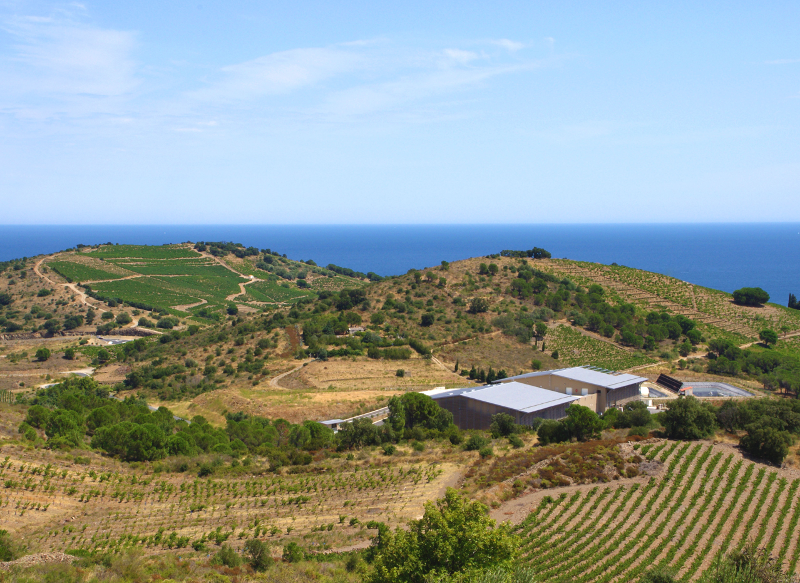
\includegraphics[height=2.5cm]{img/coop_viti} ~
    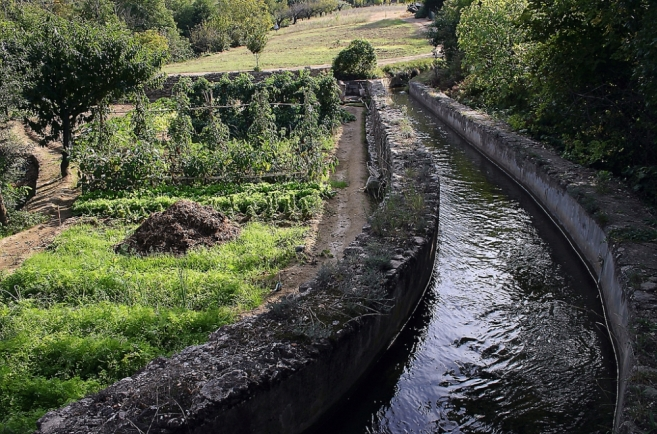
\includegraphics[height=2.5cm]{img/coop_canal}~
    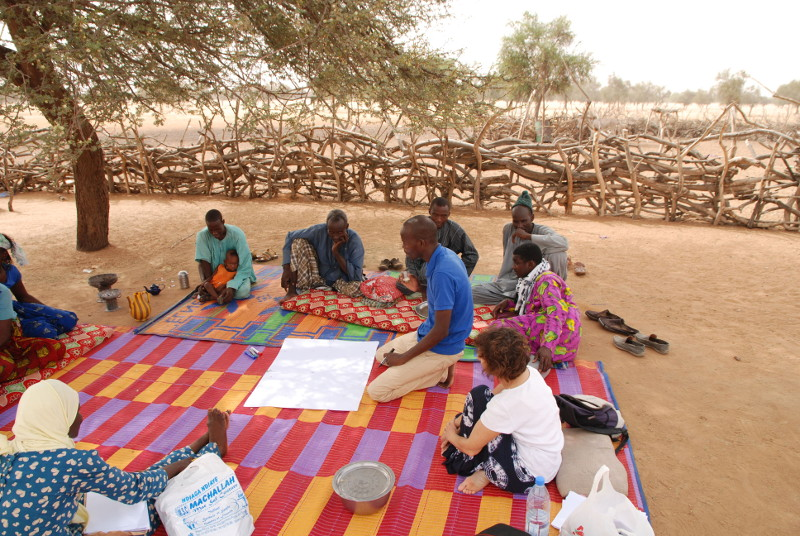
\includegraphics[height=2.5cm]{img/coop_peuls}
  \end{figure}
\end{frame}

%-=-=-=-=-=-=-=-=-=-=-=-=-=-=-=-=-=-=-=-=-=-=-=-=
%	FRAME: Un chercheur
%-=-=-=-=-=-=-=-=-=-=-=-=-=-=-=-=-=-=-=-=-=-=-=-=

\begin{frame}{\textit{Modus operandi}}
  \vspace{-2em}
	Ce qui m'amènera :
	\vspace{-1em}
	\begin{itemize}
		\item \textbf{d'un point de vue théorique} : à continuer à explorer le lien entre participation et simulation $\rightarrow$ questionner le réalisme (ex. Delay 2015),
		\item \textbf{d'un point de vue méthodologique} : à participer à l'enrichissement des outils et concepts 
\includegraphics[width=1.5cm]{img/logo_commod} $\rightarrow$ outils d'évaluation (ex. Delay et Maraud 2017).
	\end{itemize}
  %\vspace{-2em}
	Une prédilection pour la participation et la prospective :
  \begin{figure}
   	\centering
   		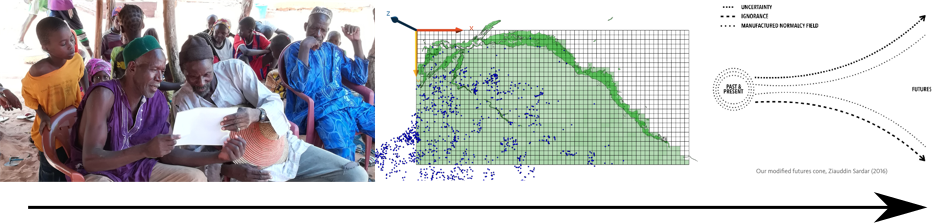
\includegraphics[width=\textwidth]{img/prespective}
  \end{figure}

\end{frame}
%-=-=-=-=-=-=-=-=-=-=-=-=-=-=-=-=-=-=-=-=-=-=-=-=
%	FRAME: LES DEFIS A RELEVER
%-=-=-=-=-=-=-=-=-=-=-=-=-=-=-=-=-=-=-=-=-=-=-=-=

\begin{frame}[c]{Les défis à relever}
\vspace{-2em}
%Dans l'étude et l'analyse des processus de développement des espaces ruraux, 3 verrous à lever :
	\begin{itemize}
		\item Représenter des \alert{\color{sthlmBlue}comportements humains hétérogènes} à l'origine d'un contrôle distribué,
		\item modéliser des \alert{interactions} au sein et entre les \alert{composantes écologiques et sociales} se produisant à différents niveaux d'organisation et d'\alert{échelles spatio-temporelles},
		\item tester la robustesse des modèles en dépit des \alert{\color{sthlmBlue}lacunes de connaissance} sur les fonctionnements biophysiques et sociaux, et sur les facteurs exogènes (climat, marché).
	\end{itemize}
  \begin{figure}
 			\centering
 				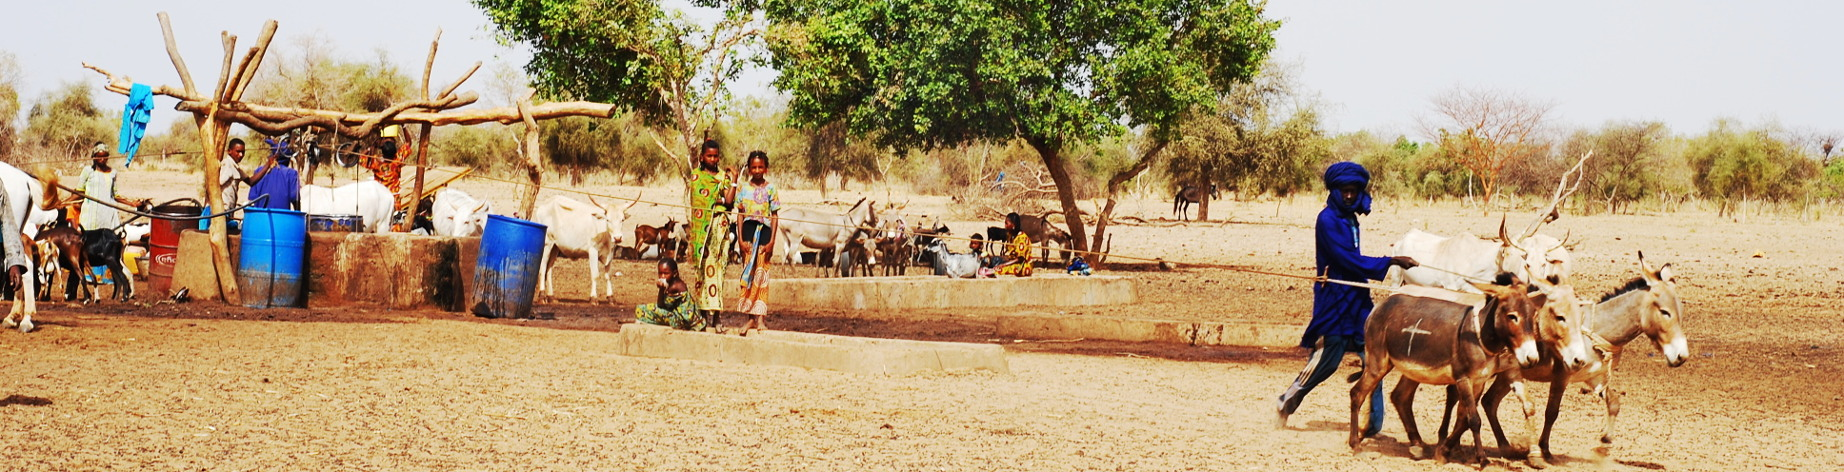
\includegraphics[width=\textwidth]{img/puis_ranerou.JPG}
	\end{figure}

\end{frame}

%-=-=-=-=-=-=-=-=-=-=-=-=-=-=-=-=-=-=-=-=-=-=-=-=
%	FRAME: Un chercheur
%-=-=-=-=-=-=-=-=-=-=-=-=-=-=-=-=-=-=-=-=-=-=-=-=

\begin{frame}{Pour relever ces défis : les outils}
	\vspace{-2em}
  Il faudra :
	\vspace{-1em}
	\begin{itemize}
		\item \textbf{d'un point de vue théorique} : formaliser des connaissances vernaculaires en langage informatique,
		\item \textbf{d'un point de vue méthodologique} : tirer parti des outils développés dans l'unité : \includegraphics[height=0.4cm]{img/logo_cormas}
\includegraphics[height=0.4cm]{img/logo_pharo}.
	\end{itemize}
  %\vspace{-1em}
	\small{
		\begin{exampleblock}{\textsc{Geographe $\neq$ Informaticien} et pourtant !}
		Un usage intensif des outils et langages de programmation :
    \vspace{-1em}
			\begin{itemize}
				\item de simulation individu centré : 
\includegraphics[height=0.4cm]{img/netlogo_icon} 
\includegraphics[height=0.4cm]{img/logo_gama}
				\item d'analyse de sensibilité : 
\includegraphics[height=0.4cm]{img/logo_openmole}, Slurm, pbs
				\item de la programmation statistique avec 
\includegraphics[width=0.5cm]{img/Rlogo}
				\item de l'information géographique : 
\includegraphics[height=0.4cm]{img/logo_qgis}, 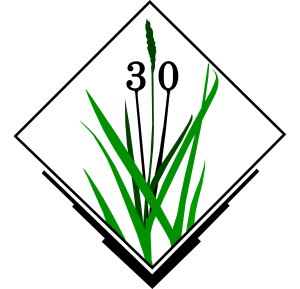
\includegraphics[height=0.4cm]{img/logo_grass}, 
\includegraphics[width=0.8cm]{img/Logo_OSGeo}
			\end{itemize}
		\end{exampleblock}
	}
\end{frame}

%-=-=-=-=-=-=-=-=-=-=-=-=-=-=-=-=-=-=-=-=-=-=-=-=
%	FRAME: L'INTEGRATION AU SENEGAL
%-=-=-=-=-=-=-=-=-=-=-=-=-=-=-=-=-=-=-=-=-=-=-=-=

\begin{frame}{Intégration dans des projets Sci. au Sénégal}
	\vspace{-2em}
    Le Sahel : croissance démographique, pauvreté, incertitudes climatiques, concurrence forte pour les ressources (eau et espace).
  	\begin{itemize}
      \item Questionnements : peut-il y avoir coexistence entre :
      \begin{itemize}
        \item Espaces pastoraux et espace cultivés/irrigués ?
        \item Agriculture familiale et agro-industrie?
      \end{itemize}
      \item Objectifs :
      \begin{itemize}
        \item \textbf{Produire des connaissances} $\rightarrow$ définition de politiques de développement durable sur les territoires semi-arides.
        \item \textbf{Accompagner la prospective} $\rightarrow$ proposer des \textit{scenarii} de gestion intégrée de l'espace.
      \end{itemize}
  	\end{itemize}
    \vspace{-1em}
    %\small{Mobiliser 
\includegraphics[width=1.5cm]{img/logo_commod} dans le cadre des programmes GITES. Utiliser ces reflexions pour enrichir BRACED.}
  % GITE : Initiative Gestion Intégrée des Territoires En zones Sèches
  % BRACED : Building Resilience and Adaptation to Climate Extremes and Disasters (BRACED) Programme porté par acting for life.
  \begin{figure}
    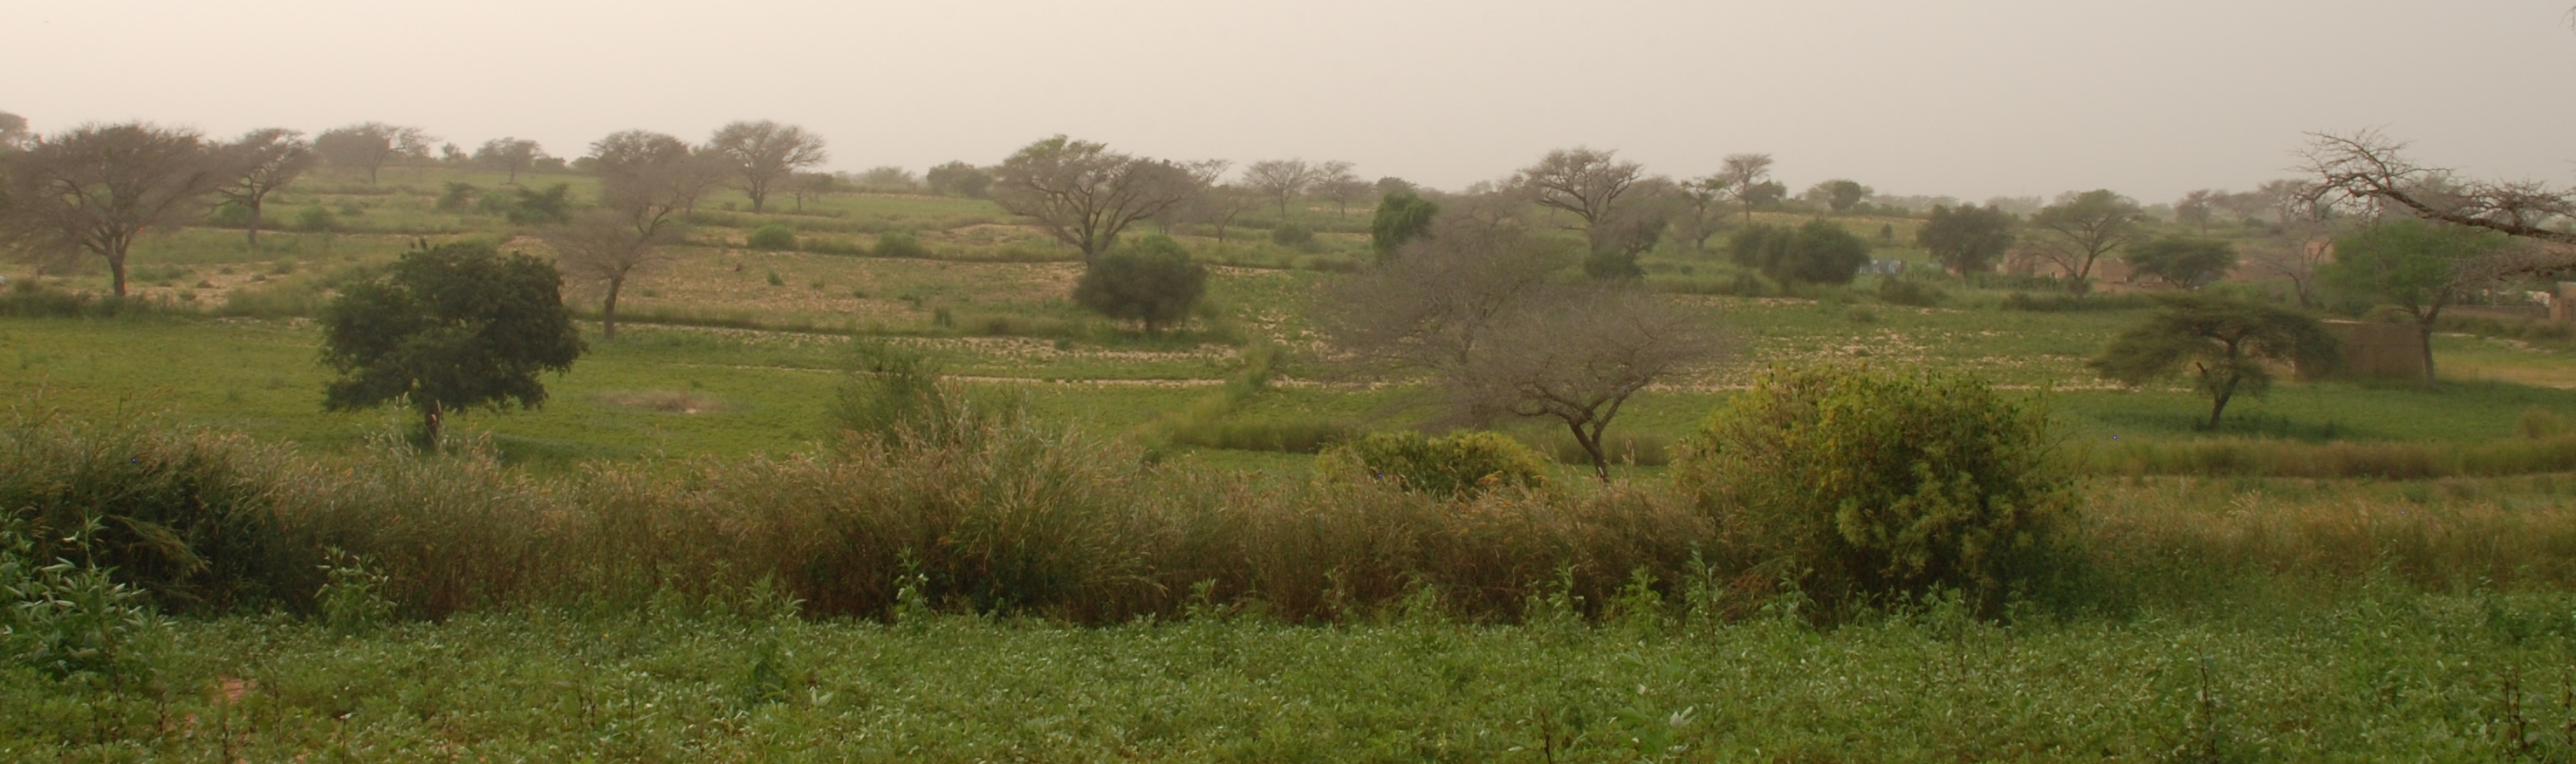
\includegraphics[width=\textwidth]{img/agri_pasto}
  \end{figure}
\end{frame}

%-=-=-=-=-=-=-=-=-=-=-=-=-=-=-=-=-=-=-=-=-=-=-=-=
%	FRAME: Temporalité
%-=-=-=-=-=-=-=-=-=-=-=-=-=-=-=-=-=-=-=-=-=-=-=-=

\begin{frame}{Ma vision dans le temps}
	\vspace{-2em}
	\small
	\begin{itemize}
		\vspace{-0.5em}
		\item après 6 mois :
		\vspace{-0.5em}
			\begin{itemize}
				\item Maîtrise des outils métiers de l'unité : \includegraphics[height=0.4cm]{img/logo_cormas}
\includegraphics[height=0.4cm]{img/logo_pharo}
				\item Mobilisation de mon réseau de collaborateurs pour la constitution de projets de recherche
        \item Proj. GITES : \alert{\color{sthlmBlue}coopération} agro-industrie/agri. familliale.
        % GITE : Initiative Gestion Intégrée des Territoires En zones Sèches
        % BRACED : Building Resilience and Adaptation to Climate Extremes and Disasters (BRACED) Programme porté par acting for life.
			\end{itemize}
		\vspace{-0.5em}
		\item après 1 an :
		\vspace{-0.5em}
			\begin{itemize}
				\item Connaissance de l'équipe d'accueil et appropriation des problématiques pour l'expatriation (PPZS - Sénégal)
				\item Mobilisation de mon réseau sur un COST-Action
        \item Développer des méthodes d'analyse de sensibilité adaptées à \includegraphics[width=1.3cm]{img/logo_commod}
        \item participation active de recherche et formation
			\end{itemize}
		\vspace{-0.5em}
		\item après 5 ans
		\vspace{-0.5em}
			\begin{itemize}
				%\item \alert{spatialisation de Nash et Pareto}
				\item indice spatial \alert{\color{sthlmBlue}interaction positive} / \alert{\color{sthlmBlue}coopération sociale} (gradients spatiaux ?)
        \item Habilitation à Diriger des Recherches (HDR) : coopération et gestion des ressources naturelles.
			\end{itemize}
	\end{itemize}
	\normalsize
\end{frame}

%-=-=-=-=-=-=-=-=-=-=-=-=-=-=-=-=-=-=-=-=-=-=-=-=
%
%	SECTION: CONCLUSION
%
%-=-=-=-=-=-=-=-=-=-=-=-=-=-=-=-=-=-=-=-=-=-=-=-=
\section{Conclusion}

%-=-=-=-=-=-=-=-=-=-=-=-=-=-=-=-=-=-=-=-=-=-=-=-=
%	FRAME: CONCLUSION 1
%-=-=-=-=-=-=-=-=-=-=-=-=-=-=-=-=-=-=-=-=-=-=-=-=

% \begin{frame}[c]{Conclusion}
% \vspace{-2em}
% {\small
% \begin{block}{\textsc{Atouts}}
% 	\vspace{-1em}
% 	\begin{itemize}
% 		\item Géographe et modélisateur → interface facilitée entre les disciplines.
% 		\item Un réseau de collaborations interdisciplinaires, inter-institutionnelles et internationales.
% 		\item Familier aux différents contextes agricoles (pastoralisme, agriculture familiale, coopération agricole, arboriculture, agriculture irriguée).
% 	\end{itemize}
% \end{block}
% \vspace{-1em}
% \begin{alertblock}{Competences}
% 	\vspace{-1em}
% 	\begin{itemize}
% 		\item Maîtrise des SMA, analyse de sensibilité, couplage de modèles, statistiques \includegraphics[width=0.5cm]{img/Rlogo}, géomatique \includegraphics[width=0.8cm]{img/Logo_OSGeo}.
% 		\item Entretien, animation de jeux sérieux, approche de modélisation d'accompagnement
% 	\end{itemize}
% \end{alertblock}
% }
% \end{frame}
%-=-=-=-=-=-=-=-=-=-=-=-=-=-=-=-=-=-=-=-=-=-=-=-=
%	FRAME: CONCLUSION 2
%-=-=-=-=-=-=-=-=-=-=-=-=-=-=-=-=-=-=-=-=-=-=-=-=
\begin{frame}[c]{Conclusion}
\vspace{-2em}
  \begin{figure}
    \centering
    \includegraphics[height=8cm]{img/widou}~
    \includegraphics[height=8cm]{img/atouts}
  \end{figure}
\end{frame}


%-=-=-=-=-=-=-=-=-=-=-=-=-=-=-=-=-=-=-=-=-=-=-=-=
%	FRAME: MERCI DE VOTRE ATTENTION
%-=-=-=-=-=-=-=-=-=-=-=-=-=-=-=-=-=-=-=-=-=-=-=-=
\begin{frame}[c]{Synthèse des activités passées}
\vspace{-2em}
\begin{minipage}{0.45\textwidth}\raggedleft
\begin{itemize}
  \small{
  \item \textbf{Resp. projet} : 3 (MAPS10, ChOICE, COMMONS),
  \item \textbf{Participation projet} : 7 (Univ., INRA, CNRS),
  \item \textbf{Annim. Ateliers et Ecole Thém.} : 3 (MAPS, LACCAVE),
  \item \textbf{Enseignement} : 80h (L,M),
  \item \textbf{Développement} : 3 (\includegraphics[height=0.6cm]{img/logo_openmole}, GamaR, OSGeo)}
\end{itemize}
\end{minipage}
\noindent\begin{minipage}{0.5\textwidth}% adapt widths of minipages to your needs
\includegraphics[width=6.5cm]{img/publication_pie}
\end{minipage}%

\end{frame}

%{
% %\usebackgroundtemplate{\includegraphics[width=1.05\paperwidth]{img/bw_fin.jpg}}%
% \usebackgroundtemplate{\includegraphics[width=1.05\paperwidth]{img/fin_diapo}}%
% \begin{frame}
%   \begin{minipage}[t][.8\textheight]{\textwidth}
%     %\color{\cnGrey}{\LARGE{Merci de votre attention}}
%
%     \vfill
%
%     %\hfill \small{Crédit photo : Thomas Misnyovszki sur Flick'r}
%     \hfill \color{\cnGrey}{\LARGE{Merci de votre attention}}
%
%     \hfill \small{Atelier participatif : Sakal 2017}
%   \end{minipage}
%
% \end{frame}
% }

%%-=-=-=-=-=-=-=-=-=-=-=-=-=-=-=-=-=-=-=-=-=-=-=-=================
%%	FIN DU DIAPORAMA OFFICIEL
%%-=-=-=-=-=-=-=-=-=-=-=-=-=-=-=-=-=-=-=-=-=-=-=-=================
%
%-=-=-=-=-=-=-=-=-=-=-=-=-=-=-=-=-=-=-=-=-=-=-=-=
%
%	SECTION: ANNEXES
%
%-=-=-=-=-=-=-=-=-=-=-=-=-=-=-=-=-=-=-=-=-=-=-=-=
%\section{Annexes}
%-=-=-=-=-=-=-=-=-=-=-=-=-=-=-=-=-=-=-=-=-=-=-=-=
%	FRAME: Exemple sur un cas concret
%-=-=-=-=-=-=-=-=-=-=-=-=-=-=-=-=-=-=-=-=-=-=-=-=
%
% \begin{frame}[c]{Cas concret : coopération, production agricole/spatiale}
% \vspace{-2em}
% L'exemple du modèle \textit{AcidityGIS} Banyuls -- Collioure.
% \vspace{-1em}
% \begin{figure}
%  			\centering
%  				\includegraphics[width=0.8\textwidth]{img/viticulture_perspective}
% 	\end{figure}
% 	\begin{itemize}
% 		\item Construction et co-construction d'un ou plusieurs modèles (\textsc{Funtowicz} et \textsc{Ravets} 1993; \textsc{Etienne} \textit{et al.} 2010).
% 		\item Évaluation -- validation des processus.
% 		\item Favoriser l'appropriation par les acteurs des modèles.
% 	\end{itemize}
%
% \end{frame}
% %-=-=-=-=-=-=-=-=-=-=-=-=-=-=-=-=-=-=-=-=-=-=-=-=
% %	FRAME: ACCOMPAGNER LE CHANGEMENT
% %-=-=-=-=-=-=-=-=-=-=-=-=-=-=-=-=-=-=-=-=-=-=-=-=
%
% \begin{frame}{Accompagner le changement}
% 	\vspace{-2em}
% 	\begin{figure}
%  			\centering
%  				\subfigure{\includegraphics[width=0.45\textwidth]{img/positionnement_modeles_echelles}}
%  				\subfigure{\includegraphics[width=0.45\textwidth]{img/path_model}}
% 	\end{figure}
% \end{frame}

\end{document}
